\chapter{Structural heterogeneities}
\label{ch:structure}

\section{Crystal-like order}
\label{sec:X_order}

\subsection{Presence and nature}

Following \citet{Kawasaki2010}, we look for crystal-like order in our system using the coarse grained \ac{BOO} method~\citep{Lechner2008} (see \SectionRef{sec:cgBOO}). The coarse grained $Q_6$ is the best parameter to distinguish between random or aperiodic structures on the one hand (low $Q_6$ values) and on the other hand local structures presenting crystal-like symmetry (high $Q_6$ values). The coarse grained $Q_4$ differentiates well between three possible types of crystal structures: \ac{BCC}, \ac{HCP} and \ac{FCC} are ranked by increasing values of $Q_4$. 

We plotted the structure populations of our experimental system (polydispersity $\Delta \approx 6\%$ but not Gaussian, as explained in \SectionRef{subsec:colloids}) in the $(Q_4, Q_6)$-plane in \FigureRef{fig:sc_Q4Q6}. As expected, normal liquid distribution is confined in the low-$Q_6$, low-$Q_4$ corner of the map. Crossing the crystallisation volume fraction $\phi_X$ we see a thickening of the tail toward high values of Q6, indicating a tendency towards crystal-like ordering in the supercooled liquid. This tendency stays the same in the range of volume fractions where the system is metastable to the coexistence regime. However, the tendency toward crystallization grows drastically when approaching the glass transition. Near $\phi_g$, the bond orientational order $Q_6$ reaches sometimes values that could be compatible with fully crystalline ordering (which is not the case, as we will see in \SectionRef{sec:density_X}).

\begin{figure}
	\centering
	\def\svgwidth{\textwidth}
	\input{Q4Q6quarter.pdf_tex}
	\caption{Population maps of our experimental system ($\Delta \approx 6\%$) in the $(Q_4, Q_6)$ plane. The color scale indicates the frequency of appearance of each structure. The volume fraction is increasing from right to left and top to bottom. Top-left: limit of supercooling close to $\phi_X$. Top-right: Metastable to fluid-solid coexistence. Bottom-left: Metastable to crystal, close to $\phi_m$. Bottom-right: Approaching the glass transition. Note that the population density is indicated in (arbitrary) log scale: most of the particles have no hint of periodic structure and abide by the normal liquid distribution, even at very low supercooling.}
	\label{fig:sc_Q4Q6}
\end{figure}

According to \FigureRef{fig:sc_Q4Q6}, normal liquid particles almost never reach values of $Q_6$ superior to $0.25$ whereas supercooled liquid do. We use this convenient threshold value $Q_6^{mrco} = 0.25$ to distinguish the crystal-like bond ordered particles often dubbed \acf{MRCO}~\citep{Shintani2006, tanaka2010critical}. For a visualisation in space of these ordered particles, see \FigureRef{fig:mrco_alphabonds}.

Particles presenting high values of $Q_6$ have moderate or high values of $Q_4$. The high $Q_6$ and low $Q_4$ corner of the symmetry map, that would indicate \ac{BCC} type of order, is empty. From the $(Q_4, Q_6)$-map, we can deduce that \ac{BCC} order is not present in our system. This confirms Kawasaki's simulation result: hard spheres or short ranged repulsive potentials do not form \ac{BCC} order.

Only looking at the $(Q_4, Q_6)$-map, it is difficult to tell apart the two remaining possible crystal-like orders: medium values of $Q_4$ may indicate well formed \ac{HCP} order or very local \ac{FCC} order surrounded by fluid-like particles. $W_4$ is a better parameter because it is positive for \ac{HCP} and negative for \ac{FCC} (and \ac{BCC}). Knowing that we have no \ac{BCC} in our system, we can safely use a $(W_4, Q_6)$-map to differentiate \ac{FCC} (top left), \ac{HCP} (top right) and aperiodic structures (bottom). The population maps presented in \FigureRef{fig:sc_W4Q6} indicates that at low supercooling, the bond order does not differentiate between \ac{HCP} and \ac{FCC}: the distribution extends toward moderate values of $Q_6$ uniformly in $W_4$. However, at deep supercooling, higher values of $Q_6$ appear only for $W_4<0$, indicating a clear preference for \ac{FCC}-like ordering. This is coherent with experiments~\citep{Gasser2001a} and simulations~\citep{Volkov2002} of crystallized hard-sphere: \ac{FCC} is the dominant order but it is often mixed with \ac{HCP} in the so called \ac{RHCP} stacking. Nevertheless, it is significant to observe that this tendency exists even before crystallisation occurs, in the mere fluctuations of the bond order.

\begin{figure}
	\centering
	\def\svgwidth{\textwidth}
	\input{W4Q6quarter.pdf_tex}
	\caption{Population maps of our experimental system in the $(W_4, Q_6)$ plane with increasing supercooling. Upon supercooling the distribution skews toward high values of $Q_6$ but uniformly along the $W_4$ axis. The preference for \acs{FCC} appears only at deep supercooling.}
	\label{fig:sc_W4Q6}
\end{figure}

We also check the other coarse grained parameters: $Q_8$ is strongly correlated to $Q_6$ (even more thant $Q_4$) and $Q_{10}$ has very low values, which indicates once again that no \ac{BCC} order exist in our system. No other significant periodic structure could be detected.

\subsection{Density and local volume}
\label{sec:density_X}

Crystallisation is a first order phase transition. If the bond order we detect was due to crystal nucleation, we would expect to observe a density excess positively correlated with the high values of bond order. \citet{tanaka2010critical} showed that in their simulations the static scattering function $S(q)$ presented little excess scattering in the low-$q$ region, indicating that there is almost no two-body density correlation on the length scale of the fluctuations of $Q_6$. 

To test this hypothesis further, we calculated the volume $V(i)$ of the Voronoi cell of each particle~\citep{Rycroft2006, rycroft2007multiscale}. We could then compute a local pseudo-volume fraction $\tilde{\phi}_{local}(i) \equiv \frac{\pi\sigma_{eff}^3}{6 V(i)}$ by assuming the same size for each particle. The average $\tilde{\phi}_{local}$ for a given value of $Q_6$ is plotted function of $Q_6$ on \FigureRef{fig:vol_Q6} (top).

\begin{figure}
	\centering
	\resizebox{\textwidth}{!}{% GNUPLOT: LaTeX picture with Postscript
\begingroup
  \makeatletter
  \providecommand\color[2][]{%
    \GenericError{(gnuplot) \space\space\space\@spaces}{%
      Package color not loaded in conjunction with
      terminal option `colourtext'%
    }{See the gnuplot documentation for explanation.%
    }{Either use 'blacktext' in gnuplot or load the package
      color.sty in LaTeX.}%
    \renewcommand\color[2][]{}%
  }%
  \providecommand\includegraphics[2][]{%
    \GenericError{(gnuplot) \space\space\space\@spaces}{%
      Package graphicx or graphics not loaded%
    }{See the gnuplot documentation for explanation.%
    }{The gnuplot epslatex terminal needs graphicx.sty or graphics.sty.}%
    \renewcommand\includegraphics[2][]{}%
  }%
  \providecommand\rotatebox[2]{#2}%
  \@ifundefined{ifGPcolor}{%
    \newif\ifGPcolor
    \GPcolortrue
  }{}%
  \@ifundefined{ifGPblacktext}{%
    \newif\ifGPblacktext
    \GPblacktexttrue
  }{}%
  % define a \g@addto@macro without @ in the name:
  \let\gplgaddtomacro\g@addto@macro
  % define empty templates for all commands taking text:
  \gdef\gplbacktext{}%
  \gdef\gplfronttext{}%
  \makeatother
  \ifGPblacktext
    % no textcolor at all
    \def\colorrgb#1{}%
    \def\colorgray#1{}%
  \else
    % gray or color?
    \ifGPcolor
      \def\colorrgb#1{\color[rgb]{#1}}%
      \def\colorgray#1{\color[gray]{#1}}%
      \expandafter\def\csname LTw\endcsname{\color{white}}%
      \expandafter\def\csname LTb\endcsname{\color{black}}%
      \expandafter\def\csname LTa\endcsname{\color{black}}%
      \expandafter\def\csname LT0\endcsname{\color[rgb]{1,0,0}}%
      \expandafter\def\csname LT1\endcsname{\color[rgb]{0,1,0}}%
      \expandafter\def\csname LT2\endcsname{\color[rgb]{0,0,1}}%
      \expandafter\def\csname LT3\endcsname{\color[rgb]{1,0,1}}%
      \expandafter\def\csname LT4\endcsname{\color[rgb]{0,1,1}}%
      \expandafter\def\csname LT5\endcsname{\color[rgb]{1,1,0}}%
      \expandafter\def\csname LT6\endcsname{\color[rgb]{0,0,0}}%
      \expandafter\def\csname LT7\endcsname{\color[rgb]{1,0.3,0}}%
      \expandafter\def\csname LT8\endcsname{\color[rgb]{0.5,0.5,0.5}}%
    \else
      % gray
      \def\colorrgb#1{\color{black}}%
      \def\colorgray#1{\color[gray]{#1}}%
      \expandafter\def\csname LTw\endcsname{\color{white}}%
      \expandafter\def\csname LTb\endcsname{\color{black}}%
      \expandafter\def\csname LTa\endcsname{\color{black}}%
      \expandafter\def\csname LT0\endcsname{\color{black}}%
      \expandafter\def\csname LT1\endcsname{\color{black}}%
      \expandafter\def\csname LT2\endcsname{\color{black}}%
      \expandafter\def\csname LT3\endcsname{\color{black}}%
      \expandafter\def\csname LT4\endcsname{\color{black}}%
      \expandafter\def\csname LT5\endcsname{\color{black}}%
      \expandafter\def\csname LT6\endcsname{\color{black}}%
      \expandafter\def\csname LT7\endcsname{\color{black}}%
      \expandafter\def\csname LT8\endcsname{\color{black}}%
    \fi
  \fi
  \setlength{\unitlength}{0.0500bp}%
  \begin{picture}(7200.00,5040.00)%
    \gplgaddtomacro\gplbacktext{%
      \csname LTb\endcsname%
      \put(1056,2520){\makebox(0,0)[r]{\strut{}$0.4$}}%
      \put(1056,3165){\makebox(0,0)[r]{\strut{}$0.5$}}%
      \put(1056,3809){\makebox(0,0)[r]{\strut{}$0.6$}}%
      \put(1056,4454){\makebox(0,0)[r]{\strut{}$0.7$}}%
      \put(1188,2300){\makebox(0,0){\strut{}}}%
      \put(1931,2300){\makebox(0,0){\strut{}}}%
      \put(2674,2300){\makebox(0,0){\strut{}}}%
      \put(3417,2300){\makebox(0,0){\strut{}}}%
      \put(4160,2300){\makebox(0,0){\strut{}}}%
      \put(4903,2300){\makebox(0,0){\strut{}}}%
      \put(5646,2300){\makebox(0,0){\strut{}}}%
      \put(6389,2300){\makebox(0,0){\strut{}}}%
      \put(418,3648){\rotatebox{-270}{\makebox(0,0){\strut{}$<\tilde{\phi}_{local}>$}}}%
      \put(6979,3648){\rotatebox{-270}{\makebox(0,0){\strut{}}}}%
      \put(3974,4666){\makebox(0,0){\strut{}}}%
      \put(3974,4665){\makebox(0,0){\strut{}}}%
      \put(264,2410){\makebox(0,0)[l]{\strut{}}}%
    }%
    \gplgaddtomacro\gplfronttext{%
      \put(5424,4603){\makebox(0,0){\strut{}Experiments}}%
      \csname LTb\endcsname%
      \put(5805,3569){\makebox(0,0)[r]{\strut{}$\phi=0.497$}}%
      \csname LTb\endcsname%
      \put(5805,3833){\makebox(0,0)[r]{\strut{}$\phi=0.535$}}%
      \csname LTb\endcsname%
      \put(5805,4097){\makebox(0,0)[r]{\strut{}$\phi=0.555$}}%
      \csname LTb\endcsname%
      \put(5805,4361){\makebox(0,0)[r]{\strut{}$\phi=0.576$}}%
    }%
    \gplgaddtomacro\gplbacktext{%
      \csname LTb\endcsname%
      \put(1056,704){\makebox(0,0)[r]{\strut{}$0.4$}}%
      \put(1056,1223){\makebox(0,0)[r]{\strut{}$0.5$}}%
      \put(1056,1741){\makebox(0,0)[r]{\strut{}$0.6$}}%
      \put(1056,2260){\makebox(0,0)[r]{\strut{}$0.7$}}%
      \put(1188,484){\makebox(0,0){\strut{}$0$}}%
      \put(1931,484){\makebox(0,0){\strut{}$0.1$}}%
      \put(2674,484){\makebox(0,0){\strut{}$0.2$}}%
      \put(3417,484){\makebox(0,0){\strut{}$0.3$}}%
      \put(4160,484){\makebox(0,0){\strut{}$0.4$}}%
      \put(4903,484){\makebox(0,0){\strut{}$0.5$}}%
      \put(5646,484){\makebox(0,0){\strut{}$0.6$}}%
      \put(6389,484){\makebox(0,0){\strut{}$0.7$}}%
      \put(418,1611){\rotatebox{-270}{\makebox(0,0){\strut{}$<\phi_{local}>$}}}%
      \put(6979,1611){\rotatebox{-270}{\makebox(0,0){\strut{}}}}%
      \put(3974,154){\makebox(0,0){\strut{}$Q_6$}}%
      \put(3974,2409){\makebox(0,0){\strut{}}}%
      \put(3974,2408){\makebox(0,0){\strut{}}}%
      \put(264,110){\makebox(0,0)[l]{\strut{}}}%
    }%
    \gplgaddtomacro\gplfronttext{%
      \put(5358,2346){\makebox(0,0){\strut{}Simulations}}%
      \csname LTb\endcsname%
      \put(5805,1048){\makebox(0,0)[r]{\strut{}$\phi=0.487$ }}%
      \csname LTb\endcsname%
      \put(5805,1312){\makebox(0,0)[r]{\strut{}$\phi=0.507$ }}%
      \csname LTb\endcsname%
      \put(5805,1576){\makebox(0,0)[r]{\strut{}$\phi=0.528$ }}%
      \csname LTb\endcsname%
      \put(5805,1840){\makebox(0,0)[r]{\strut{}$\phi=0.548$ }}%
      \csname LTb\endcsname%
      \put(5805,2104){\makebox(0,0)[r]{\strut{}$\phi=0.568$ }}%
    }%
    \gplbacktext
    \put(0,0){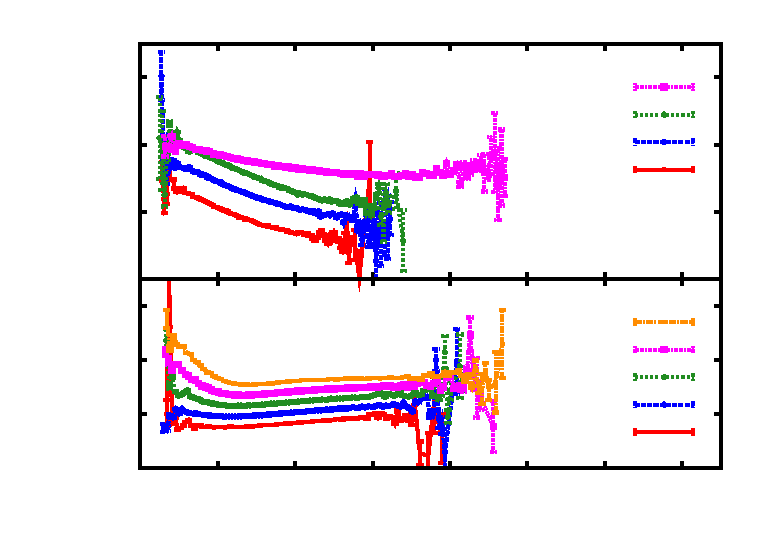
\includegraphics{phi_Q6_xpsim}}%
    \gplfronttext
  \end{picture}%
\endgroup
}
	\caption{Local Voronoi volume fraction $\tilde{\phi}_{local}$ function of $Q_6$ for various volume fractions. In experiments (top), the particles with a crystal-like bond order have more local free volume than the non-crystalline particles. In simulations (bottom), the local volume fraction is almost constant for moderate and high values of $Q_6$. However, low value of $Q_6$ present a clear excess of local volume fraction.}
	\label{fig:vol_Q6}
\end{figure}

We observe that the local volume fraction \emph{decreases} in average with increasing $Q_6$ at all volume fractions $\phi$. This clearly shows that the bond-ordered particles are not crystal nuclei. Moreover, this result shades new light on the driving force of bond ordering: the particles self organise in order to maximize their local free volume.

To confirm this result, we performed the same type of calculation on Kawasaki's simulation data ($\Delta=6\%$). Here, we have access to the precise diameter of each particle, so we computed the radical Voronoi tessellation that weights the position of the cell boundaries according to the relative radii of the particles, yielding a cell volume $V_{radical}(i)\neq V(i)$ in general. When computing the local volume fraction, we also used the real volume of each particle. 
\begin{equation}
\phi_{local}(i) \equiv \frac{\pi\sigma(i)}{6 V_{radical}(i)}
\end{equation}
Actually, the influence of such a refinement proved to be negligible. The result is plotted on \FigureRef{fig:vol_Q6} (bottom). The trend is somewhat different in simulation: the local volume fraction is almost flat but slightly rising from moderate ($0.15$) to high $Q_6$. This supports the idea that the high $Q_6$ region are not crystal nuclei. However the role of local free volume as the driving force of the ordering is less clear. We also note a strong excess of local volume fraction at low $Q_6$; excess that is more and more pronounced with increasing overall volume fraction. The behaviour at low $Q_6$ will be explained in \SectionRef{sec:ico_volume}.

To monitor the density difference between high-$Q_6$ particles and their environment, we coarse-grained the volume fraction over the first shell. No sensible difference could be observed between this neighbourhood volume fraction and the local volume fraction of the crystalline bond ordered particles.


\subsection{Spatial extent}
\label{sec:mrco_spatial}

The size of the crystal-like ordered regions grows with increasing density, as displayed in \FigureRef{fig:mrco_alphabonds}. To characterise the spatial extent of the crystal-like bond order, we use $G_6(r)$, the spatial correlation of the tensorial order parameter $Q_{6 m}$ defined in \SectionRef{sec:cgBOO}. The difference between the $g_6(r)$ and $G_6(r)$ is displayed in \FigureRef{fig:G6}: $g_6(r)$ caches all 6-fold bond order and is oscillating between positive and negative values; whereas $G_6(r)$ (sensible only to the crystal-like order) stays positive over a few inter-particle distances. The valleys in $G_6(r)$ corresponds to the valleys of the \ac{RDF}. Particles that are between two shells are analogue to off-lattice particles in a crystal: although few, they have a high probability of being disordered. What actually describes the correlation of crystal-like bond order in the upper envelope of $G_6(r)$.

\begin{figure}
	\centering
	\subfloat[No coarse graining]{\label{fig:g6}\resizebox{0.5\textwidth}{!}{\begin{Large}% GNUPLOT: LaTeX picture with Postscript
\begingroup
  \makeatletter
  \providecommand\color[2][]{%
    \GenericError{(gnuplot) \space\space\space\@spaces}{%
      Package color not loaded in conjunction with
      terminal option `colourtext'%
    }{See the gnuplot documentation for explanation.%
    }{Either use 'blacktext' in gnuplot or load the package
      color.sty in LaTeX.}%
    \renewcommand\color[2][]{}%
  }%
  \providecommand\includegraphics[2][]{%
    \GenericError{(gnuplot) \space\space\space\@spaces}{%
      Package graphicx or graphics not loaded%
    }{See the gnuplot documentation for explanation.%
    }{The gnuplot epslatex terminal needs graphicx.sty or graphics.sty.}%
    \renewcommand\includegraphics[2][]{}%
  }%
  \providecommand\rotatebox[2]{#2}%
  \@ifundefined{ifGPcolor}{%
    \newif\ifGPcolor
    \GPcolortrue
  }{}%
  \@ifundefined{ifGPblacktext}{%
    \newif\ifGPblacktext
    \GPblacktexttrue
  }{}%
  % define a \g@addto@macro without @ in the name:
  \let\gplgaddtomacro\g@addto@macro
  % define empty templates for all commands taking text:
  \gdef\gplbacktext{}%
  \gdef\gplfronttext{}%
  \makeatother
  \ifGPblacktext
    % no textcolor at all
    \def\colorrgb#1{}%
    \def\colorgray#1{}%
  \else
    % gray or color?
    \ifGPcolor
      \def\colorrgb#1{\color[rgb]{#1}}%
      \def\colorgray#1{\color[gray]{#1}}%
      \expandafter\def\csname LTw\endcsname{\color{white}}%
      \expandafter\def\csname LTb\endcsname{\color{black}}%
      \expandafter\def\csname LTa\endcsname{\color{black}}%
      \expandafter\def\csname LT0\endcsname{\color[rgb]{1,0,0}}%
      \expandafter\def\csname LT1\endcsname{\color[rgb]{0,1,0}}%
      \expandafter\def\csname LT2\endcsname{\color[rgb]{0,0,1}}%
      \expandafter\def\csname LT3\endcsname{\color[rgb]{1,0,1}}%
      \expandafter\def\csname LT4\endcsname{\color[rgb]{0,1,1}}%
      \expandafter\def\csname LT5\endcsname{\color[rgb]{1,1,0}}%
      \expandafter\def\csname LT6\endcsname{\color[rgb]{0,0,0}}%
      \expandafter\def\csname LT7\endcsname{\color[rgb]{1,0.3,0}}%
      \expandafter\def\csname LT8\endcsname{\color[rgb]{0.5,0.5,0.5}}%
    \else
      % gray
      \def\colorrgb#1{\color{black}}%
      \def\colorgray#1{\color[gray]{#1}}%
      \expandafter\def\csname LTw\endcsname{\color{white}}%
      \expandafter\def\csname LTb\endcsname{\color{black}}%
      \expandafter\def\csname LTa\endcsname{\color{black}}%
      \expandafter\def\csname LT0\endcsname{\color{black}}%
      \expandafter\def\csname LT1\endcsname{\color{black}}%
      \expandafter\def\csname LT2\endcsname{\color{black}}%
      \expandafter\def\csname LT3\endcsname{\color{black}}%
      \expandafter\def\csname LT4\endcsname{\color{black}}%
      \expandafter\def\csname LT5\endcsname{\color{black}}%
      \expandafter\def\csname LT6\endcsname{\color{black}}%
      \expandafter\def\csname LT7\endcsname{\color{black}}%
      \expandafter\def\csname LT8\endcsname{\color{black}}%
    \fi
  \fi
  \setlength{\unitlength}{0.0500bp}%
  \begin{picture}(7200.00,5040.00)%
    \gplgaddtomacro\gplbacktext{%
      \csname LTb\endcsname%
      \put(1188,704){\makebox(0,0)[r]{\strut{}$-0.03$}}%
      \put(1188,1156){\makebox(0,0)[r]{\strut{}$-0.02$}}%
      \put(1188,1609){\makebox(0,0)[r]{\strut{}$-0.01$}}%
      \put(1188,2061){\makebox(0,0)[r]{\strut{}$0$}}%
      \put(1188,2514){\makebox(0,0)[r]{\strut{}$0.01$}}%
      \put(1188,2966){\makebox(0,0)[r]{\strut{}$0.02$}}%
      \put(1188,3419){\makebox(0,0)[r]{\strut{}$0.03$}}%
      \put(1188,3871){\makebox(0,0)[r]{\strut{}$0.04$}}%
      \put(1188,4324){\makebox(0,0)[r]{\strut{}$0.05$}}%
      \put(1188,4776){\makebox(0,0)[r]{\strut{}$0.06$}}%
      \put(1320,484){\makebox(0,0){\strut{}$0$}}%
      \put(1864,484){\makebox(0,0){\strut{}$1$}}%
      \put(2408,484){\makebox(0,0){\strut{}$2$}}%
      \put(2952,484){\makebox(0,0){\strut{}$3$}}%
      \put(3496,484){\makebox(0,0){\strut{}$4$}}%
      \put(4040,484){\makebox(0,0){\strut{}$5$}}%
      \put(4584,484){\makebox(0,0){\strut{}$6$}}%
      \put(5128,484){\makebox(0,0){\strut{}$7$}}%
      \put(5672,484){\makebox(0,0){\strut{}$8$}}%
      \put(6216,484){\makebox(0,0){\strut{}$9$}}%
      \put(6760,484){\makebox(0,0){\strut{}$10$}}%
      \put(286,2740){\rotatebox{-270}{\makebox(0,0){\strut{}$g_6(r)$}}}%
      \put(6979,2740){\rotatebox{-270}{\makebox(0,0){\strut{}}}}%
      \put(4040,154){\makebox(0,0){\strut{}$r/\sigma$}}%
      \put(4040,4666){\makebox(0,0){\strut{}}}%
      \put(4040,4665){\makebox(0,0){\strut{}}}%
      \put(132,110){\makebox(0,0)[l]{\strut{}}}%
    }%
    \gplgaddtomacro\gplfronttext{%
      \csname LTb\endcsname%
      \put(5773,1922){\makebox(0,0)[r]{\strut{}$\phi=0.497$}}%
      \csname LTb\endcsname%
      \put(5773,1592){\makebox(0,0)[r]{\strut{}$\phi=0.535$}}%
      \csname LTb\endcsname%
      \put(5773,1262){\makebox(0,0)[r]{\strut{}$\phi=0.555$}}%
      \csname LTb\endcsname%
      \put(5773,932){\makebox(0,0)[r]{\strut{}$\phi=0.576$}}%
    }%
    \gplgaddtomacro\gplbacktext{%
      \csname LTb\endcsname%
      \put(3348,3071){\makebox(0,0)[r]{\strut{}$10^{-5}$}}%
      \put(3348,3798){\makebox(0,0)[r]{\strut{}$10^{-3}$}}%
      \put(3348,4524){\makebox(0,0)[r]{\strut{}$10^{-1}$}}%
      \put(4026,2488){\makebox(0,0){\strut{}$2$}}%
      \put(4619,2488){\makebox(0,0){\strut{}$4$}}%
      \put(5213,2488){\makebox(0,0){\strut{}$6$}}%
      \put(5806,2488){\makebox(0,0){\strut{}$8$}}%
      \put(6400,2488){\makebox(0,0){\strut{}$10$}}%
      \put(6619,3616){\rotatebox{-270}{\makebox(0,0){\strut{}}}}%
      \put(4940,4414){\makebox(0,0){\strut{}}}%
      \put(4940,4413){\makebox(0,0){\strut{}}}%
      \put(2028,2378){\makebox(0,0)[l]{\strut{}}}%
    }%
    \gplgaddtomacro\gplfronttext{%
    }%
    \gplbacktext
    \put(0,0){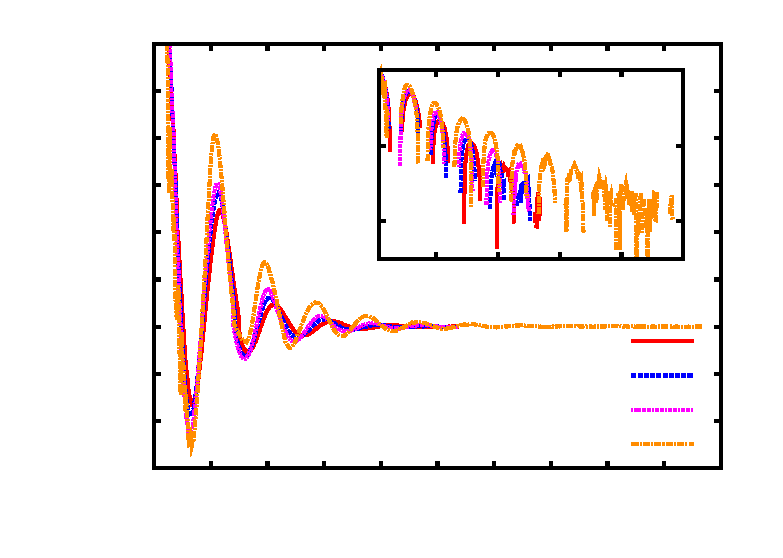
\includegraphics{g6}}%
    \gplfronttext
  \end{picture}%
\endgroup
\end{Large}}}
	\subfloat[With coarse graining]{\label{fig:fit_G6}\resizebox{0.5\textwidth}{!}{\begin{Large}% GNUPLOT: LaTeX picture with Postscript
\begingroup
  \makeatletter
  \providecommand\color[2][]{%
    \GenericError{(gnuplot) \space\space\space\@spaces}{%
      Package color not loaded in conjunction with
      terminal option `colourtext'%
    }{See the gnuplot documentation for explanation.%
    }{Either use 'blacktext' in gnuplot or load the package
      color.sty in LaTeX.}%
    \renewcommand\color[2][]{}%
  }%
  \providecommand\includegraphics[2][]{%
    \GenericError{(gnuplot) \space\space\space\@spaces}{%
      Package graphicx or graphics not loaded%
    }{See the gnuplot documentation for explanation.%
    }{The gnuplot epslatex terminal needs graphicx.sty or graphics.sty.}%
    \renewcommand\includegraphics[2][]{}%
  }%
  \providecommand\rotatebox[2]{#2}%
  \@ifundefined{ifGPcolor}{%
    \newif\ifGPcolor
    \GPcolortrue
  }{}%
  \@ifundefined{ifGPblacktext}{%
    \newif\ifGPblacktext
    \GPblacktexttrue
  }{}%
  % define a \g@addto@macro without @ in the name:
  \let\gplgaddtomacro\g@addto@macro
  % define empty templates for all commands taking text:
  \gdef\gplbacktext{}%
  \gdef\gplfronttext{}%
  \makeatother
  \ifGPblacktext
    % no textcolor at all
    \def\colorrgb#1{}%
    \def\colorgray#1{}%
  \else
    % gray or color?
    \ifGPcolor
      \def\colorrgb#1{\color[rgb]{#1}}%
      \def\colorgray#1{\color[gray]{#1}}%
      \expandafter\def\csname LTw\endcsname{\color{white}}%
      \expandafter\def\csname LTb\endcsname{\color{black}}%
      \expandafter\def\csname LTa\endcsname{\color{black}}%
      \expandafter\def\csname LT0\endcsname{\color[rgb]{1,0,0}}%
      \expandafter\def\csname LT1\endcsname{\color[rgb]{0,1,0}}%
      \expandafter\def\csname LT2\endcsname{\color[rgb]{0,0,1}}%
      \expandafter\def\csname LT3\endcsname{\color[rgb]{1,0,1}}%
      \expandafter\def\csname LT4\endcsname{\color[rgb]{0,1,1}}%
      \expandafter\def\csname LT5\endcsname{\color[rgb]{1,1,0}}%
      \expandafter\def\csname LT6\endcsname{\color[rgb]{0,0,0}}%
      \expandafter\def\csname LT7\endcsname{\color[rgb]{1,0.3,0}}%
      \expandafter\def\csname LT8\endcsname{\color[rgb]{0.5,0.5,0.5}}%
    \else
      % gray
      \def\colorrgb#1{\color{black}}%
      \def\colorgray#1{\color[gray]{#1}}%
      \expandafter\def\csname LTw\endcsname{\color{white}}%
      \expandafter\def\csname LTb\endcsname{\color{black}}%
      \expandafter\def\csname LTa\endcsname{\color{black}}%
      \expandafter\def\csname LT0\endcsname{\color{black}}%
      \expandafter\def\csname LT1\endcsname{\color{black}}%
      \expandafter\def\csname LT2\endcsname{\color{black}}%
      \expandafter\def\csname LT3\endcsname{\color{black}}%
      \expandafter\def\csname LT4\endcsname{\color{black}}%
      \expandafter\def\csname LT5\endcsname{\color{black}}%
      \expandafter\def\csname LT6\endcsname{\color{black}}%
      \expandafter\def\csname LT7\endcsname{\color{black}}%
      \expandafter\def\csname LT8\endcsname{\color{black}}%
    \fi
  \fi
  \setlength{\unitlength}{0.0500bp}%
  \begin{picture}(7200.00,5040.00)%
    \gplgaddtomacro\gplbacktext{%
      \csname LTb\endcsname%
      \put(1056,704){\makebox(0,0)[r]{\strut{}$10^{-7}$}}%
      \put(1056,1518){\makebox(0,0)[r]{\strut{}$10^{-6}$}}%
      \put(1056,2333){\makebox(0,0)[r]{\strut{}$10^{-5}$}}%
      \put(1056,3147){\makebox(0,0)[r]{\strut{}$10^{-4}$}}%
      \put(1056,3962){\makebox(0,0)[r]{\strut{}$10^{-3}$}}%
      \put(1056,4776){\makebox(0,0)[r]{\strut{}$10^{-2}$}}%
      \put(1453,484){\makebox(0,0){\strut{}$2$}}%
      \put(2117,484){\makebox(0,0){\strut{}$2.5$}}%
      \put(2780,484){\makebox(0,0){\strut{}$3$}}%
      \put(3443,484){\makebox(0,0){\strut{}$3.5$}}%
      \put(4107,484){\makebox(0,0){\strut{}$4$}}%
      \put(4770,484){\makebox(0,0){\strut{}$4.5$}}%
      \put(5433,484){\makebox(0,0){\strut{}$5$}}%
      \put(6097,484){\makebox(0,0){\strut{}$5.5$}}%
      \put(6760,484){\makebox(0,0){\strut{}$6$}}%
      \put(286,2740){\rotatebox{-270}{\makebox(0,0){\strut{}$G_6(r)$}}}%
      \put(6979,2740){\rotatebox{-270}{\makebox(0,0){\strut{}}}}%
      \put(3974,154){\makebox(0,0){\strut{}$r/\sigma$}}%
      \put(3974,4666){\makebox(0,0){\strut{}}}%
      \put(3974,4665){\makebox(0,0){\strut{}}}%
      \put(-264,110){\makebox(0,0)[l]{\strut{}}}%
    }%
    \gplgaddtomacro\gplfronttext{%
      \csname LTb\endcsname%
      \put(2904,932){\makebox(0,0)[r]{\strut{}$\phi=0.535$}}%
      \csname LTb\endcsname%
      \put(2904,1262){\makebox(0,0)[r]{\strut{}$\phi=0.555$}}%
      \csname LTb\endcsname%
      \put(2904,1592){\makebox(0,0)[r]{\strut{}$\phi=0.576$}}%
    }%
    \gplbacktext
    \put(0,0){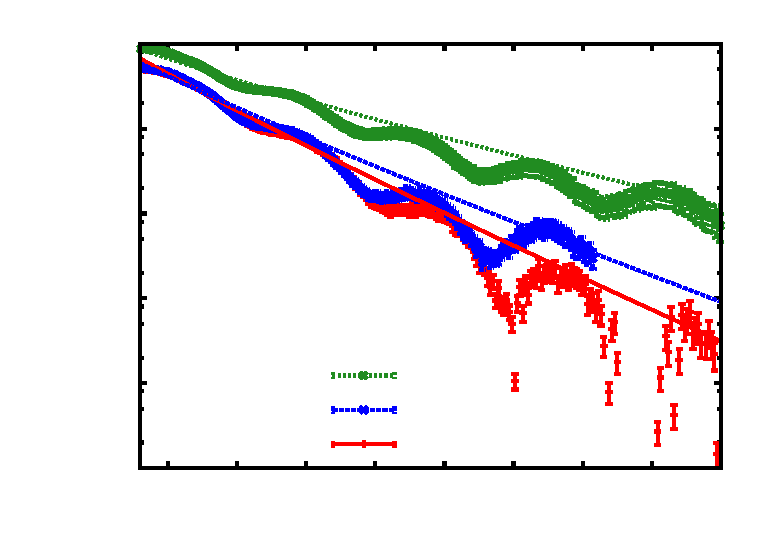
\includegraphics{fit_G6}}%
    \gplfronttext
  \end{picture}%
\endgroup
\end{Large}}}
	\caption{\subref{fig:g6} Spatial correlation of any 6-fold bond order. Inset is the same data in semi-log scale. \subref{fig:fit_G6} Correlation $G_6(r)$ of the crystal-like order. The length scale of the correlation is increasing with the volume fraction. The lines are the fit by the Orstein-Zernike function (see \EquationRef{eq:OZ}).}
	\label{fig:G6}
\end{figure}

The characteristic length of the spatial correlation obviously increases with supercooling. We characterise the decay of the bond order correlation by fitting the upper envelope of $G_6(r)$ by the Ornstein-Zernike function (Onsager formula):
\begin{equation}
	G_6(r) \propto r^{-1}\exp( -\frac{r}{\xi_6} )
	\label{eq:OZ}
\end{equation}

This correlation length increases with supercooling. The results are displayed in \FigureRef{fig:fit_xi} and will be discussed in more details in \SectionRef{sec:struct_vs_dyn}.

\section{Icosahedral order}

\subsection{Presence}

\citet{Kawasaki2010} focused only on coarse-grained bond order and thus overlooked all the possible local structures that lack periodicity. In particular, icosahedral order have been found in many types of supercooled liquids~\citep{steinhardt1983boo, Jonsson1988, Tomida1995, DiCicco2003, Coslovich2007} with isotropic attractive potentials and is even at the heart of most of the frustration-based theories of the glass transition~\citep{tarjus2005fba, Celino2007, VanMeel2009}. In addition, fragments of icosahedra have been found in densely packed hard spheres ($\phi>\phi_g$). This body of evidence made the absence of icosahedra order in polydisperse quasi-hard spheres (\acs{WCA}) rather surprising.

To look for aperiodic structures, we had to return to the non-coarse grained particle-centred invariants $(q_\ell, w_\ell)$ with $\ell=4,6,8,10$ defined in \SectionRef{sec:boo_invariants}. The structures qualified by this method are the clusters with a particle at the centre, \latin{i.e.} the one shown in \FigureRef{fig:basicClusters}. The coarse-grained analysis has already discarded \ac{BCC} and identified \ac{FCC} order and some \ac{HCP}, so we know that the crystal-like structures are well detected by the $Q_6$ parameter. Only remains the icosahedron (\FigureRef{fig:ico}), and its twisted version the dodecahedron (\FigureRef{fig:dodecahedron}).

Because of the thermal distortion of the structures, we have to choose among the bond order invariants the one that pulls the type of structure we look for out of the distribution of the other structures. In particular, parameters giving a value close to $0$ are to be avoided, like $q_4$ and $q_8$ for the icosahedron. According to \TableRef{tab:rotational_invarients}, the choice of the icosahedral order parameter is then drastically restricted: $w_4$ and $w_8$ are undefined, $q_6$ is large but close to the values of the crystals, $q_{10}$ and $w_{10}$ are surrounded by the values of other structures. \citet{steinhardt1983boo} demonstrated that $w_6$ reaches its maximum absolute value for icosahedral ordering ($w_6^ico \approx -0.169$) whereas crystals are almost zero-valued. Thus we will use $w_6$ to detect icosahedra.

\begin{figure}
	\centering
	\def\svgwidth{0.8\textwidth}
	\input{w6Q6quarter.pdf_tex}
	\caption{Population maps of our experimental system in the $(w_6, Q_6)$ plane with increasing supercooling. The green arrows mark respectively the crystallisation and the quasi-crystallisation paths.}
	\label{fig:sc_w6Q6}
\end{figure}

The $(w_6, Q_6)$-plane is a very good map to describe both crystalline (\ac{FCC}-like) and icosahedral ordering. It shows these two possible tendencies as orthogonal and pulls the perfect structures distribution out of the liquid distribution. In \FigureRef{fig:sc_w6Q6}, we plotted the population of the different structures on such a map. Contrary to the crystal-like structure, the icosahedral order is already present in the normal liquid; however, perfect icosahedra are few. With increasing density, more and more particles are detected at low $w_6$ values, indicating a growing tendency toward icosahedral order. Our $(w_6, Q_6)$ population map also emphasises the mutual exclusion between the two types of order.

An ambiguity remains about the exact nature of the structure for values larger than $w_6^{dodec} = -0.0937$ . However, the dodecahedron can be considered as a way of distorting an icosahedron and is by right somewhere in the middle of the icosahedral axis. We will not try to differentiate between the distorted icosahedra for $w_6>w_6^{dodec}$, where most of the liquid particles belong. For more negative values of $w_6$, we are sure to deal with (distorted) icosahedra. For a visualisation in space of this ordered particles, see \FigureRef{fig:mrco_alphabonds}.

\begin{figure}
	\centering	
	\begin{small}%
	\tikz\shade[ball color=green!33!black] circle (0.4em);
	Crystal-like\quad%
	\tikz\shade[ball color=blue!33!black] circle (0.25em);
	Isolated icosahedra\quad%
	\tikz\shade[ball color=blue] circle (0.4em);%
	\tikz\shade[ball color=green] circle (0.4em);%
	\tikz\shade[ball color=orange] circle (0.4em);%
	\tikz\shade[ball color=red] circle (0.4em);
	Connected icosahedra%
	\end{small}\\
	\subfloat[Normal liquid ($\phi=0.497$)]{
		\label{fig:mrco_alphabonds_liq}
		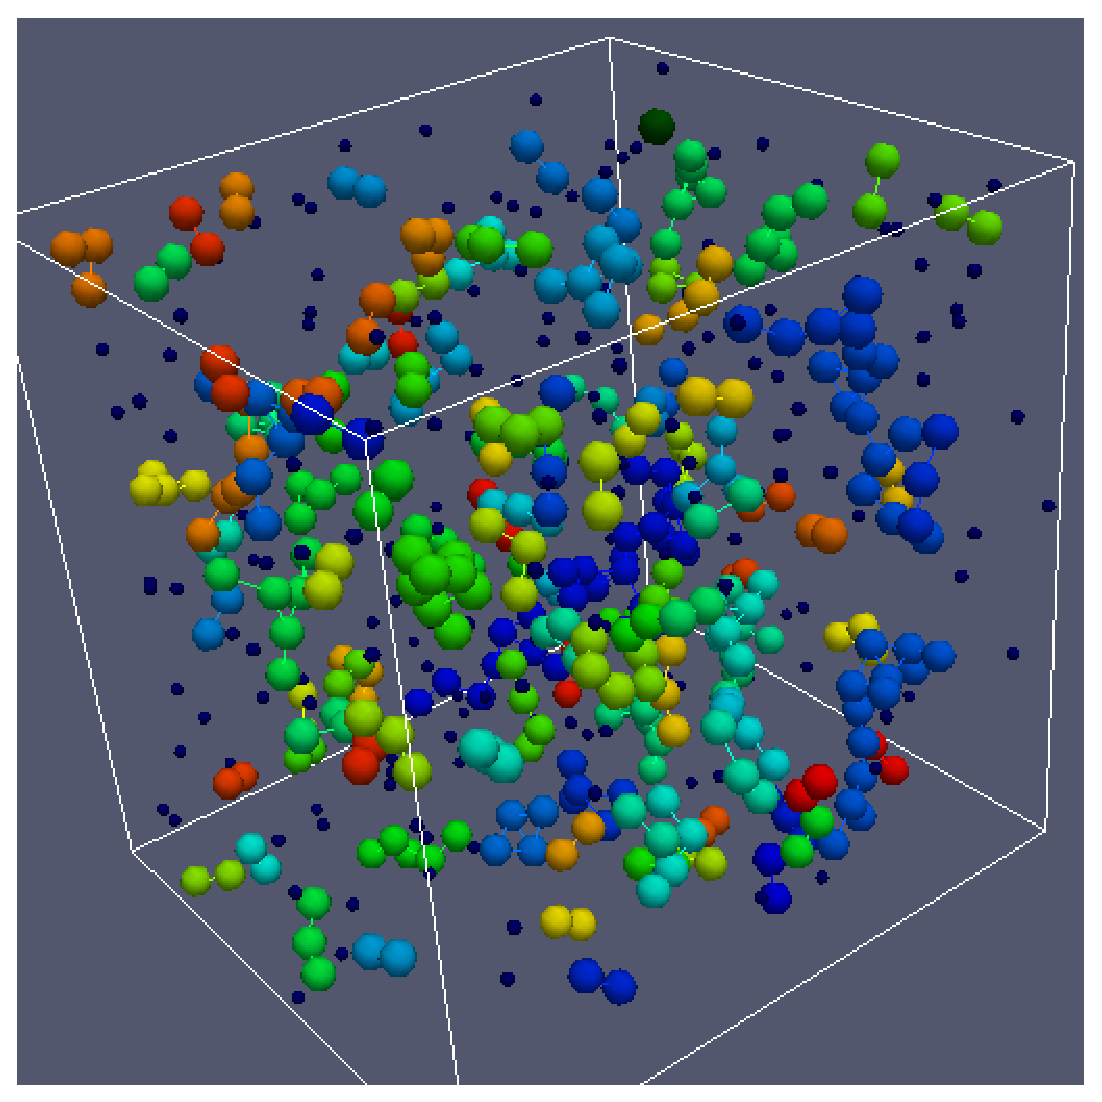
\includegraphics[width=0.4\textwidth]{mrco_alphabonds_3954}}\quad
	\subfloat[Supercooled liquid ($\phi=0.535$)]{
		\label{fig:mrco_alphabonds_sc}
		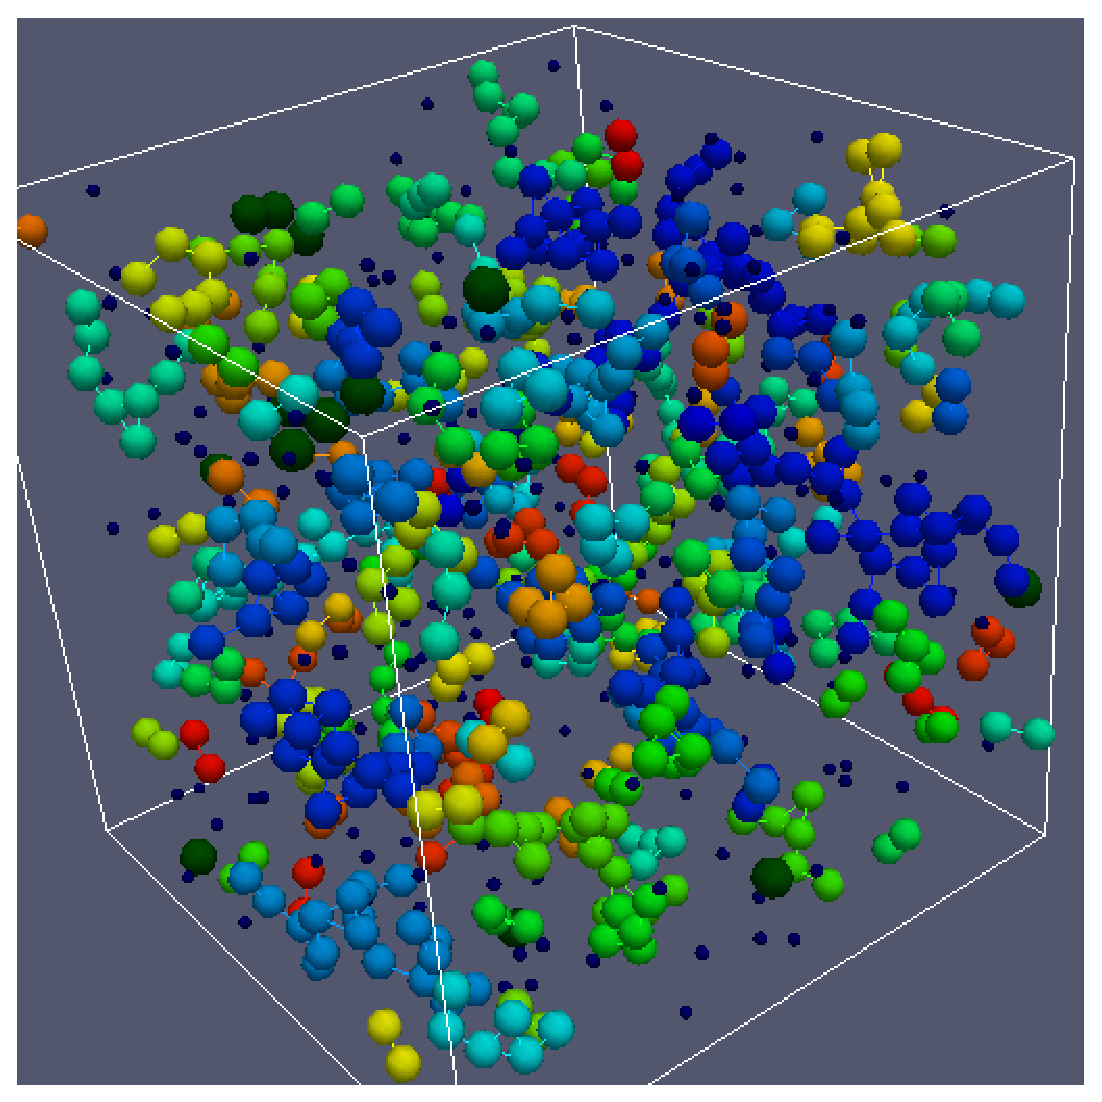
\includegraphics[width=0.4\textwidth]{mrco_alphabonds_4582}}
	\caption{Structural heterogeneities in real space. Computer reconstruction from confocal microscopy coordinates. Only the central particle of each structure is displayed for clarity. See \PageRef{fig:mrco_alphabonds_deep}.}
\end{figure}
\begin{figure}
	\ContinuedFloat
	\centering
	\begin{small}%
	\tikz\shade[ball color=green!33!black] circle (0.4em);
	Crystal-like\quad%
	\tikz\shade[ball color=blue!33!black] circle (0.25em);
	Isolated icosahedra\quad%
	\tikz\shade[ball color=blue] circle (0.4em);%
	\tikz\shade[ball color=green] circle (0.4em);%
	\tikz\shade[ball color=orange] circle (0.4em);%
	\tikz\shade[ball color=red] circle (0.4em);
	Connected icosahedra%
	\end{small}\\
	\subfloat
		[Deeply supercooled ($\phi=0.576$). We are looking through a slice of the sample of thickness $\sim 8 \sigma$.]{
		\label{fig:mrco_alphabonds_deep}
		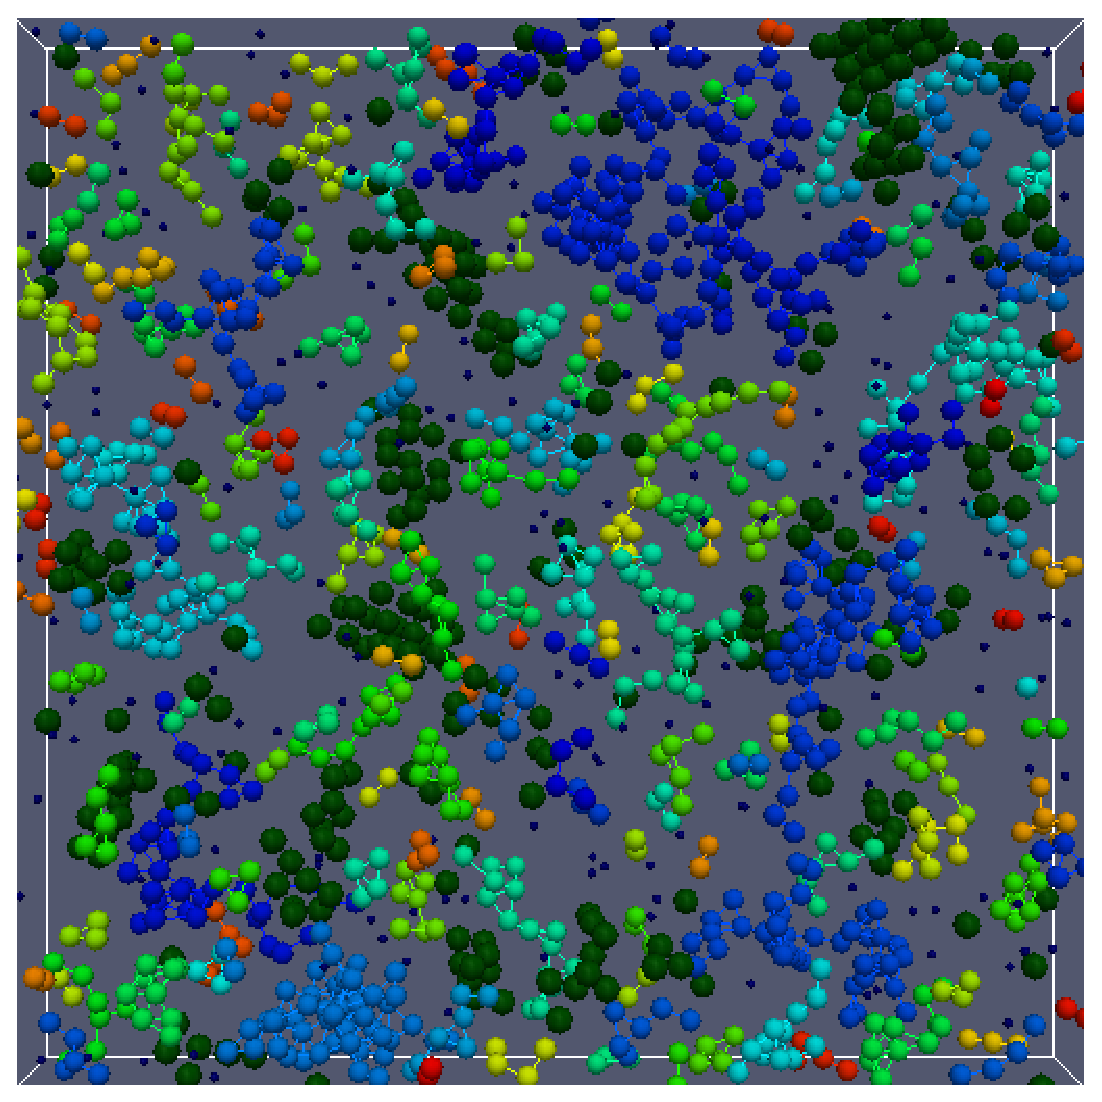
\includegraphics[width=0.8\textwidth]{mrco_alphabonds_go1}}
	\caption{Crystal-like bond orderer particles ($Q_6>Q_6^{mrco}$) are displayed in dark green. Isolated icosahedral particles ($w_6<w_6^{dodec}$) are displayed smaller and in dark blue. The lines are the bonds between neighbouring icosahedra (like in \FigureRef{ico_19}, not like in \FigureRef{ico_23}). Neighbouring icosahedra are displayed with the same bright color. Because the connection is defined within our experimental window, the percolation in 3D of the whole icosahedral network cannot be excluded and is even very probable in \subref{fig:mrco_alphabonds_deep}.}
	\label{fig:mrco_alphabonds}
\end{figure}


\subsection{Density and local volume}
\label{sec:ico_volume}
In a similar way to the crystalline order, we can characterise the local volume fraction along the icosahedral order axis. The average $\tilde{\phi}_{local}$ for a given value of $w_6$ is plotted function of $w_6$ on the left part of \FigureRef{fig:vol_w6}.

\begin{figure}
	\centering
	\resizebox{\textwidth}{!}{% GNUPLOT: LaTeX picture with Postscript
\begingroup
  \makeatletter
  \providecommand\color[2][]{%
    \GenericError{(gnuplot) \space\space\space\@spaces}{%
      Package color not loaded in conjunction with
      terminal option `colourtext'%
    }{See the gnuplot documentation for explanation.%
    }{Either use 'blacktext' in gnuplot or load the package
      color.sty in LaTeX.}%
    \renewcommand\color[2][]{}%
  }%
  \providecommand\includegraphics[2][]{%
    \GenericError{(gnuplot) \space\space\space\@spaces}{%
      Package graphicx or graphics not loaded%
    }{See the gnuplot documentation for explanation.%
    }{The gnuplot epslatex terminal needs graphicx.sty or graphics.sty.}%
    \renewcommand\includegraphics[2][]{}%
  }%
  \providecommand\rotatebox[2]{#2}%
  \@ifundefined{ifGPcolor}{%
    \newif\ifGPcolor
    \GPcolortrue
  }{}%
  \@ifundefined{ifGPblacktext}{%
    \newif\ifGPblacktext
    \GPblacktexttrue
  }{}%
  % define a \g@addto@macro without @ in the name:
  \let\gplgaddtomacro\g@addto@macro
  % define empty templates for all commands taking text:
  \gdef\gplbacktext{}%
  \gdef\gplfronttext{}%
  \makeatother
  \ifGPblacktext
    % no textcolor at all
    \def\colorrgb#1{}%
    \def\colorgray#1{}%
  \else
    % gray or color?
    \ifGPcolor
      \def\colorrgb#1{\color[rgb]{#1}}%
      \def\colorgray#1{\color[gray]{#1}}%
      \expandafter\def\csname LTw\endcsname{\color{white}}%
      \expandafter\def\csname LTb\endcsname{\color{black}}%
      \expandafter\def\csname LTa\endcsname{\color{black}}%
      \expandafter\def\csname LT0\endcsname{\color[rgb]{1,0,0}}%
      \expandafter\def\csname LT1\endcsname{\color[rgb]{0,1,0}}%
      \expandafter\def\csname LT2\endcsname{\color[rgb]{0,0,1}}%
      \expandafter\def\csname LT3\endcsname{\color[rgb]{1,0,1}}%
      \expandafter\def\csname LT4\endcsname{\color[rgb]{0,1,1}}%
      \expandafter\def\csname LT5\endcsname{\color[rgb]{1,1,0}}%
      \expandafter\def\csname LT6\endcsname{\color[rgb]{0,0,0}}%
      \expandafter\def\csname LT7\endcsname{\color[rgb]{1,0.3,0}}%
      \expandafter\def\csname LT8\endcsname{\color[rgb]{0.5,0.5,0.5}}%
    \else
      % gray
      \def\colorrgb#1{\color{black}}%
      \def\colorgray#1{\color[gray]{#1}}%
      \expandafter\def\csname LTw\endcsname{\color{white}}%
      \expandafter\def\csname LTb\endcsname{\color{black}}%
      \expandafter\def\csname LTa\endcsname{\color{black}}%
      \expandafter\def\csname LT0\endcsname{\color{black}}%
      \expandafter\def\csname LT1\endcsname{\color{black}}%
      \expandafter\def\csname LT2\endcsname{\color{black}}%
      \expandafter\def\csname LT3\endcsname{\color{black}}%
      \expandafter\def\csname LT4\endcsname{\color{black}}%
      \expandafter\def\csname LT5\endcsname{\color{black}}%
      \expandafter\def\csname LT6\endcsname{\color{black}}%
      \expandafter\def\csname LT7\endcsname{\color{black}}%
      \expandafter\def\csname LT8\endcsname{\color{black}}%
    \fi
  \fi
  \setlength{\unitlength}{0.0500bp}%
  \begin{picture}(7200.00,5040.00)%
    \gplgaddtomacro\gplbacktext{%
      \csname LTb\endcsname%
      \put(1056,2520){\makebox(0,0)[r]{\strut{}$0.4$}}%
      \put(1056,3165){\makebox(0,0)[r]{\strut{}$0.5$}}%
      \put(1056,3809){\makebox(0,0)[r]{\strut{}$0.6$}}%
      \put(1056,4454){\makebox(0,0)[r]{\strut{}$0.7$}}%
      \put(1369,2300){\makebox(0,0){\strut{}}}%
      \put(1791,2300){\makebox(0,0){\strut{}}}%
      \put(2394,2300){\makebox(0,0){\strut{}}}%
      \put(2997,2300){\makebox(0,0){\strut{}}}%
      \put(418,3648){\rotatebox{-270}{\makebox(0,0){\strut{}$<\tilde{\phi}_{local}>$}}}%
      \put(3819,3648){\rotatebox{-270}{\makebox(0,0){\strut{}}}}%
      \put(2394,4666){\makebox(0,0){\strut{}}}%
      \put(2394,4665){\makebox(0,0){\strut{}}}%
      \put(264,2190){\makebox(0,0)[l]{\strut{}}}%
    }%
    \gplgaddtomacro\gplfronttext{%
      \put(2557,4537){\makebox(0,0){\strut{}Experiments}}%
    }%
    \gplgaddtomacro\gplbacktext{%
      \csname LTb\endcsname%
      \put(3468,2520){\makebox(0,0)[r]{\strut{}}}%
      \put(3468,3165){\makebox(0,0)[r]{\strut{}}}%
      \put(3468,3809){\makebox(0,0)[r]{\strut{}}}%
      \put(3468,4454){\makebox(0,0)[r]{\strut{}}}%
      \put(3781,2300){\makebox(0,0){\strut{}}}%
      \put(4203,2300){\makebox(0,0){\strut{}}}%
      \put(4806,2300){\makebox(0,0){\strut{}}}%
      \put(5409,2300){\makebox(0,0){\strut{}}}%
      \put(6231,3648){\rotatebox{-270}{\makebox(0,0){\strut{}$<\tilde{\phi}_{ngb}>$}}}%
      \put(4806,4666){\makebox(0,0){\strut{}}}%
      \put(4806,4665){\makebox(0,0){\strut{}}}%
      \put(3336,2190){\makebox(0,0)[l]{\strut{}}}%
    }%
    \gplgaddtomacro\gplfronttext{%
      \csname LTb\endcsname%
      \put(4669,3877){\makebox(0,0)[r]{\strut{}$\phi=0.497$}}%
      \csname LTb\endcsname%
      \put(4669,4097){\makebox(0,0)[r]{\strut{}$\phi=0.535$}}%
      \csname LTb\endcsname%
      \put(4669,4317){\makebox(0,0)[r]{\strut{}$\phi=0.555$}}%
      \csname LTb\endcsname%
      \put(4669,4537){\makebox(0,0)[r]{\strut{}$\phi=0.576$}}%
    }%
    \gplgaddtomacro\gplbacktext{%
      \csname LTb\endcsname%
      \put(1056,704){\makebox(0,0)[r]{\strut{}$0.4$}}%
      \put(1056,1223){\makebox(0,0)[r]{\strut{}$0.5$}}%
      \put(1056,1741){\makebox(0,0)[r]{\strut{}$0.6$}}%
      \put(1056,2260){\makebox(0,0)[r]{\strut{}$0.7$}}%
      \put(1369,484){\makebox(0,0){\strut{}$-0.17$}}%
      \put(1791,484){\makebox(0,0){\strut{}$-0.1$}}%
      \put(2394,484){\makebox(0,0){\strut{}$0$}}%
      \put(2997,484){\makebox(0,0){\strut{}$0.1$}}%
      \put(418,1611){\rotatebox{90}{\makebox(0,0){\strut{}$<\phi_{local}>$}}}%
      \put(2394,154){\makebox(0,0){\strut{}$w_6$}}%
      \put(2394,2409){\makebox(0,0){\strut{}}}%
      \put(2394,2408){\makebox(0,0){\strut{}}}%
      \put(264,110){\makebox(0,0)[l]{\strut{}}}%
    }%
    \gplgaddtomacro\gplfronttext{%
      \put(2161,2305){\makebox(0,0){\strut{}Simulations}}%
      \csname LTb\endcsname%
      \put(2740,1865){\makebox(0,0)[r]{\strut{}$\phi=0.548$ }}%
      \csname LTb\endcsname%
      \put(2740,2085){\makebox(0,0)[r]{\strut{}$\phi=0.568$ }}%
    }%
    \gplgaddtomacro\gplbacktext{%
      \csname LTb\endcsname%
      \put(3468,704){\makebox(0,0)[r]{\strut{}}}%
      \put(3468,1223){\makebox(0,0)[r]{\strut{}}}%
      \put(3468,1741){\makebox(0,0)[r]{\strut{}}}%
      \put(3468,2260){\makebox(0,0)[r]{\strut{}}}%
      \put(3781,484){\makebox(0,0){\strut{}$-0.17$}}%
      \put(4203,484){\makebox(0,0){\strut{}$-0.1$}}%
      \put(4806,484){\makebox(0,0){\strut{}$0$}}%
      \put(5409,484){\makebox(0,0){\strut{}$0.1$}}%
      \put(6231,1611){\rotatebox{90}{\makebox(0,0){\strut{}$<\phi_{ngb}>$}}}%
      \put(4806,154){\makebox(0,0){\strut{}$w_6$}}%
      \put(4806,2409){\makebox(0,0){\strut{}}}%
      \put(4806,2408){\makebox(0,0){\strut{}}}%
      \put(3336,110){\makebox(0,0)[l]{\strut{}}}%
    }%
    \gplgaddtomacro\gplfronttext{%
      \csname LTb\endcsname%
      \put(4669,1865){\makebox(0,0)[r]{\strut{}$\phi=0.487$ }}%
      \csname LTb\endcsname%
      \put(4669,2085){\makebox(0,0)[r]{\strut{}$\phi=0.507$ }}%
      \csname LTb\endcsname%
      \put(4669,2305){\makebox(0,0)[r]{\strut{}$\phi=0.528$ }}%
    }%
    \gplbacktext
    \put(0,0){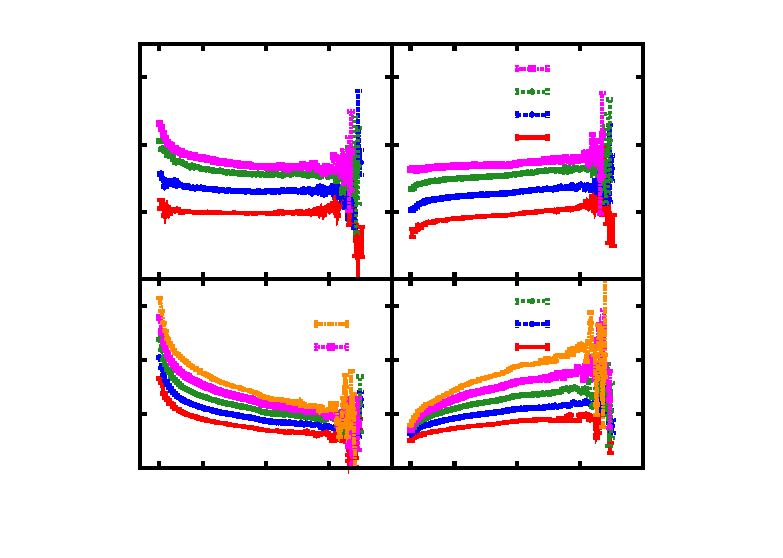
\includegraphics{phi_w6_xpsim_total}}%
    \gplfronttext
  \end{picture}%
\endgroup
}
	\caption{Left: Local Voronoi volume fraction $\phi_{local}$ as a function of $w_6$ for various overall volume fractions. In experiments (top) as in simulations (bottom), the particles with icosahedral bond order have less local free volume than the other structures. This effect is much more pronounced in the simulation.\\ Right: The same, but with $\phi_{ngb}$ the volume fraction coarse-grained on the first shell. The neighbours of a particle with icosahedral bond order have less local free volume than any other structure. This effect is much more pronounced in the simulation where the perfect icosahedra seems to have the same coarse-grained volume fraction at any overall volume fraction.}
	\label{fig:vol_w6}
\end{figure}

We observe that in the supercooled regime the local volume fraction \emph{increases} in average with increasing icosahedral order (decreasing $w_6$) at all overall volume fraction even if the effect is more subtle for the sample above the supercooling. This trend is much more pronounced in the simulation data, and is at the origin of the excess in the local volume fraction observed at low $Q_6$ in \FigureRef{fig:vol_Q6}. This result shows that the tendency toward icosahedral order can not be explained by a gain in free volume at the level of the particle. Two possible causes can be proposed:
\begin{enumerate}
	\item\label{it:ngbvol} Provided that a fraction of the system orders into dense icosahedra, the remaining particles are allowed larger free volume.
	\item\label{it:localvib} An icosahedral neighbourhood allows more vibrational modes than a random configuration, even if the local free volume is smaller.
\end{enumerate}

Hypothesis~\ref{it:localvib} cannot be tested without fine time resolution. However scenario~\ref{it:ngbvol} can be easily tested by coarse-graining the local volume over a certain length. For the appropriate length scale, the coarse-grained volume of the icosahedron should be the same or lower that a random neighbourhood. In the right part of \FigureRef{fig:vol_w6}, we coarse-grained the local volume fraction over the first shell:
\begin{equation}
	\phi_{ngb}(i) \equiv \frac{1}{{N_{ngb}(i)}}\sum_j^{N_{ngb}(i)} \phi_{local}(i)
\end{equation}

What we observe firmly confirms the scenario~\ref{it:ngbvol}: the formation of an icosahedron decreases the local free volume of the central particle but expands the local free volume of its neighbours.

In the simulations of supercooled liquid ($\phi=0.48$ excluded), the first shell volume fraction $\phi_{ngb}$ of the perfect icosahedra ($w_6 \sim W_6^{ico}$) seems to be the same for any overall volume fraction, with a value of $\phi^{ico} \simeq 0.46$. We can speculate that $\phi^{ico}$ corresponds to the volume fraction of an hypothetical quasi-crystalline phase at coexistence with the fluid. The reason why we could not observe this convergence in experiments may be due to the difference in the size distribution, more skewed toward small diameters and less able to form an iscosahedra of the same size.

In all the curves of \FigureRef{fig:vol_w6}, we observe a change of the slope at the same value of $w_6^* \simeq -0.15$, and no special feature around $w_6^{dodec}$. This may indicate a qualitative difference between "perfect" icosahedra ($w_6<w_6^*$) and distorted ones ($w_6^*<w_6<w_6^{dodec}$); the former being much more stabilized by free volume effects.

\subsection{Spatial arrangement}

How long-range is icosahedral order? $w_6$ detects only local, 13-particle icosahedra. Are they can be isolated and randomly distributed in space, or grouped together in an ordered fashion ? The former case is the most probable at low densities in our system: remember that we have no attractive potential and thus no preferred bond length; packing is what favours icosahedral ordering. The latter case should append anyway at high packing, when many icosahedra form and must themselves pack. However, unlike crystalline order, the icosahedral order cannot fill space. This means that the icosahedra cannot arrange in a compact way and should form a network, as observed by \citet{Tomida1995} for attractive particles.

Indeed, as displayed in \FigureRef{fig:mrco_alphabonds}, strings and non-compact clusters made of interconnected icosahedra form and grow larger with increasing the volume fraction. Surprisingly for hard spheres, aggregates of icosahedra are observed even before supercooling. This means that the interlocking of icosahedra is favoured even at low packing. We speculate that the gain in free volume of the \emph{neighbours} of the icosahedral particle, and the resulting gain of vibrational entropy, is the driving force of this aggregation: an isolated icosahedron has to compress its central particle, whereas the central particles of two $\alpha$-interlocking icosahedra like in \FigureRef{ico_19} are neighbours and thus benefit from each-other's free volume effect. This and the deformation intrinsic to the $\alpha$-interlocking state explains why most of the icosahedra do not reach $w_6^{ico}$.

In \FigureRef{fig:stable_ico}, we stress the localisation of the perfect icosahedra ($w_6<w_6^*$). They are mostly included in clusters of distorted icosahedra ($w_6^*<w_6<w_6^{dodec}$), not always at the core of it and not peculiarly grouped together. Without the distorted icosahedra linking them, the perfect icosahedra would not appear as a developed network but as isolated clusters much smaller in size and in number than the crystal-like bond ordered regions.

\begin{figure}
	\centering
	\begin{small}%
	\tikz\shade[ball color=blue] circle (0.4em);%
	\tikz\shade[ball color=green] circle (0.4em);%
	\tikz\shade[ball color=orange] circle (0.4em);%
	\tikz\shade[ball color=red] circle (0.4em);
	Perfect icosahedra\qquad%
	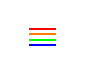
\begin{tikzpicture}
		\draw[thick, blue] (0,-0.3em) -- ++(-1em,0);
		\draw[thick, green] (0,-0.1em) -- ++(-1em,0);
		\draw[thick, orange] (0,0.1em) -- ++(-1em,0);
		\draw[thick, red] (0,0.3em) -- ++(-1em,0);
	\end{tikzpicture}
	Imperfect icosahedral network%
	\end{small}\\
	\subfloat[Normal liquid ($\phi=0.497$)]{
		\label{fig:stable_ico_liq}
		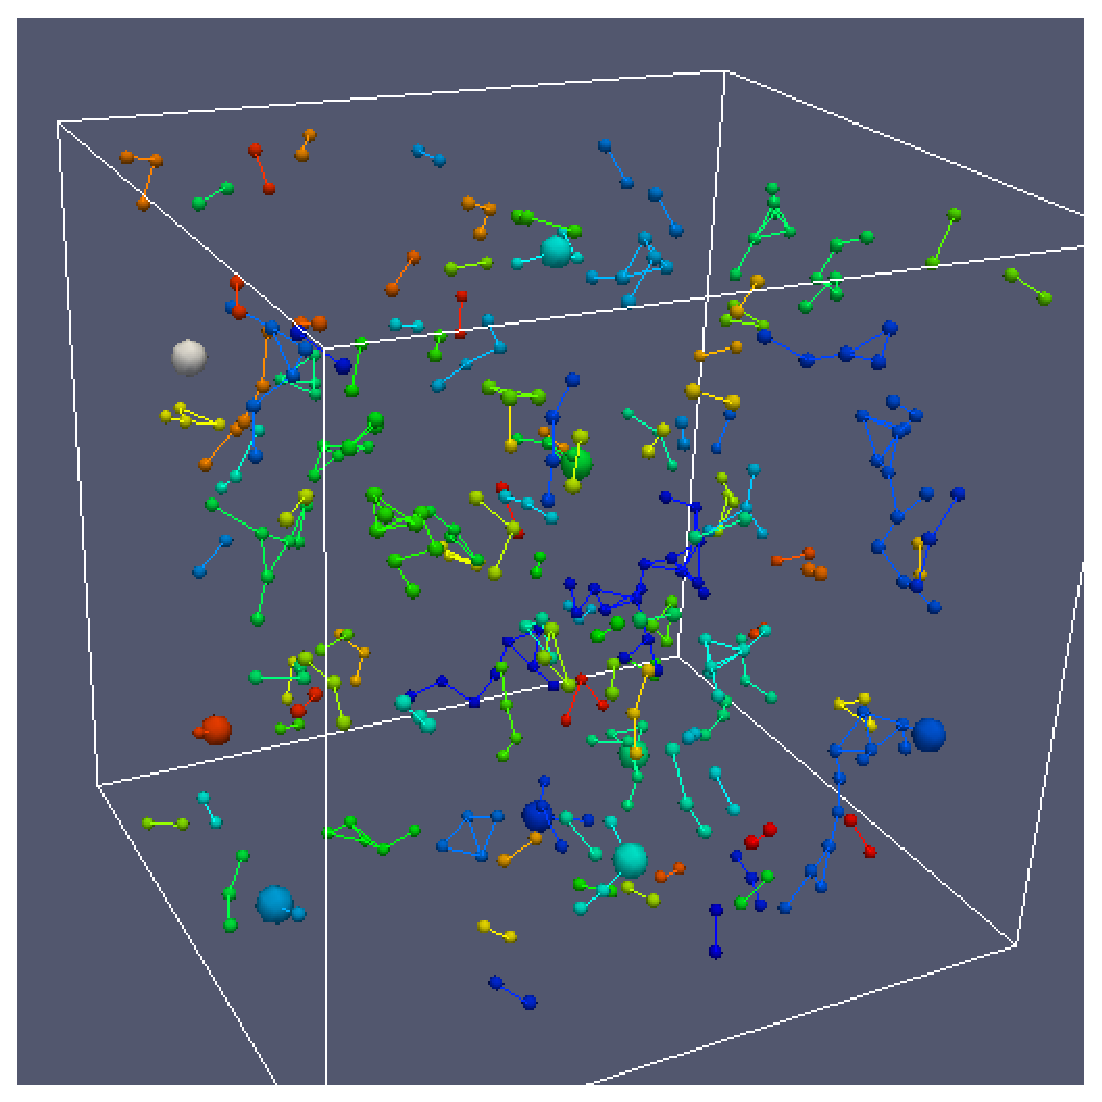
\includegraphics[width=0.4\textwidth]{stable_ico_3954}}\quad
	\subfloat[Supercooled liquid ($\phi=0.535$)]{
		\label{fig:stable_ico_sc}
		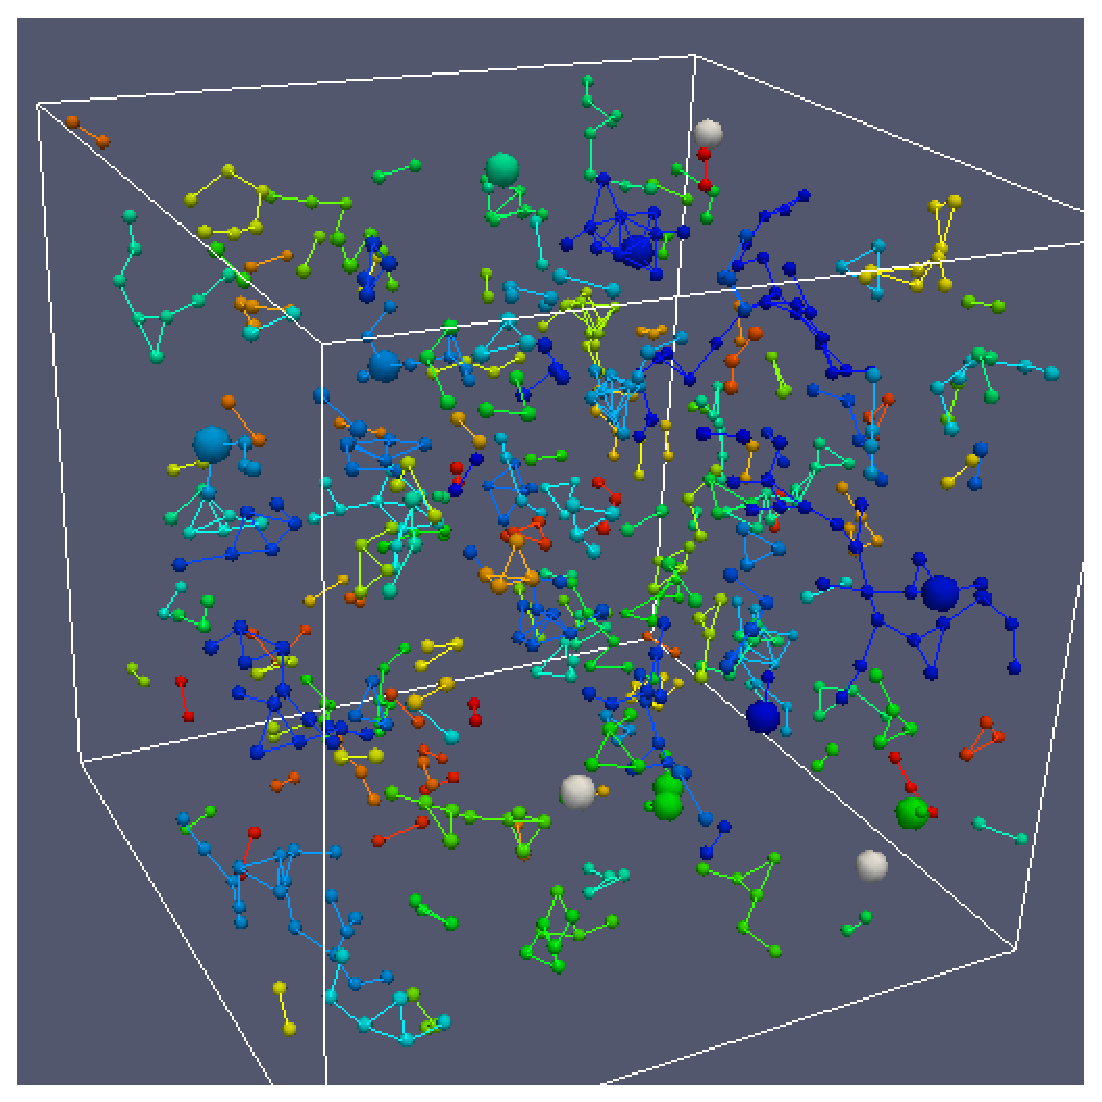
\includegraphics[width=0.4\textwidth]{stable_ico_4582}}
	\caption{Prefect and imperfect icosahedra. See \PageRef{fig:stable_ico_deep}.}
\end{figure}
\begin{figure}
	\ContinuedFloat
	\centering
	\begin{small}%
	\tikz\shade[ball color=blue] circle (0.4em);%
	\tikz\shade[ball color=green] circle (0.4em);%
	\tikz\shade[ball color=orange] circle (0.4em);%
	\tikz\shade[ball color=red] circle (0.4em);
	Perfect icosahedra\qquad%
	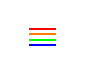
\begin{tikzpicture}
		\draw[thick, blue] (0,-0.3em) -- ++(-1em,0);
		\draw[thick, green] (0,-0.1em) -- ++(-1em,0);
		\draw[thick, orange] (0,0.1em) -- ++(-1em,0);
		\draw[thick, red] (0,0.3em) -- ++(-1em,0);
	\end{tikzpicture}
	Imperfect icosahedral network%
	\end{small}\\
	\subfloat
		[Deeply supercooled ($\phi=0.576$). We are looking through a slice of the sample of thickness $\sim 8 \sigma$.]{
		\label{fig:stable_ico_deep}
		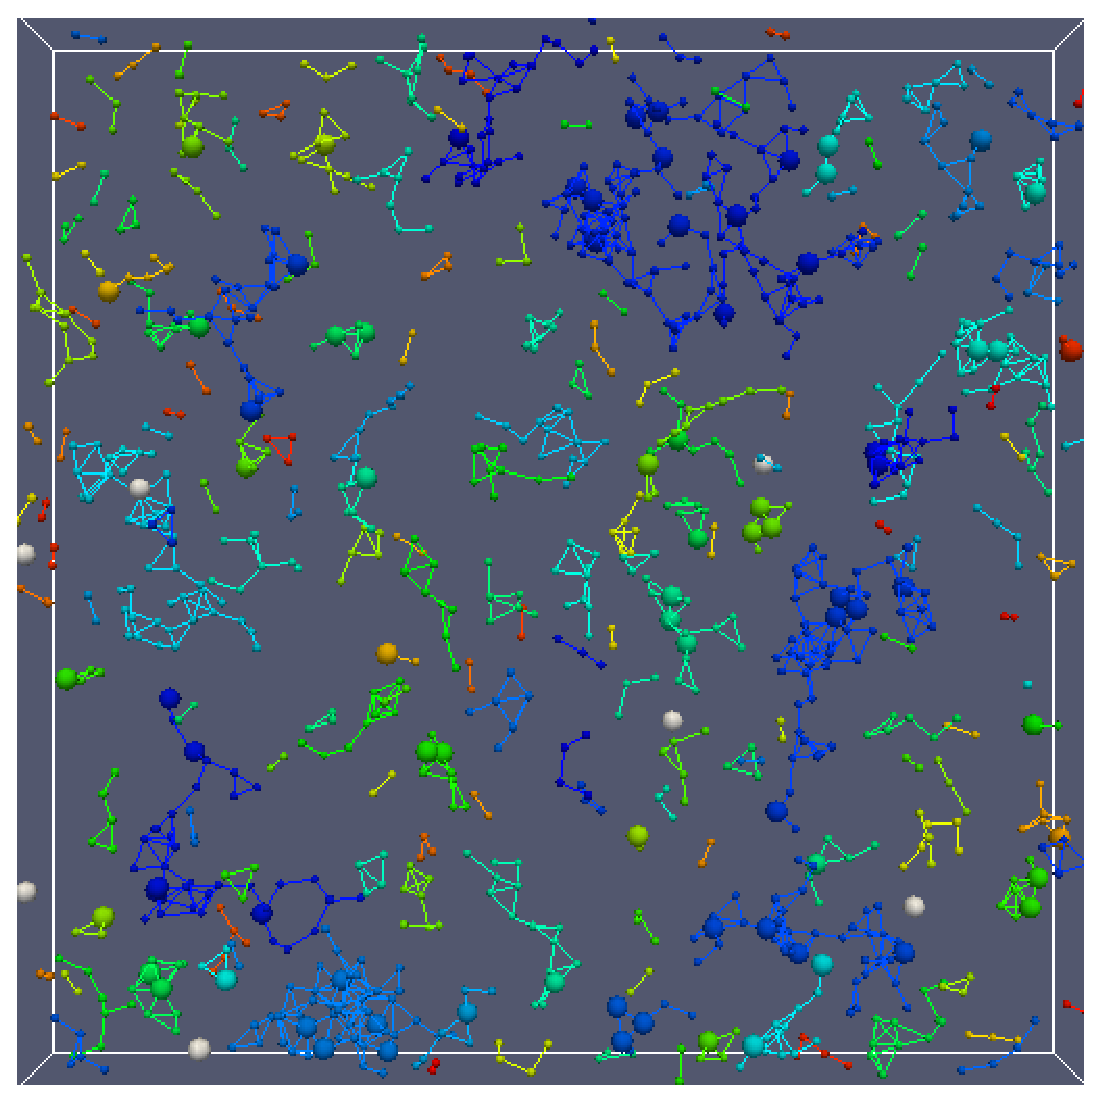
\includegraphics[width=0.8\textwidth]{stable_ico_go1}}
	\caption{The network of neighbouring icosahedral particles ($w_6<w_6^{dodec}$). The colours differentiate between disconnected icosahedral clusters. Perfect icosahedra ($w_6<w_6^*$) are represented larger than the connected distorted icosahedra ($w_6^*<w_6<w_6^{dodec}$). Isolated distorted icosahedra are not plotted.}
	\label{fig:stable_ico}
\end{figure}


\section{Lifetimes}

Which structures are stable in time? To answer this question, we compute $g_\ell(t)$, the particle-wise time autocorrelation function of the tensorial bond order parameter defined in \EquationRef{eq:boo_time_correl}, and its coarse-grained version $G_\ell(t)$. Unfortunately, the bond order is very sensitive to thermal vibrations. If $\delta t$ is the shortest time interval accessible in a given experiment, $g_\ell(\delta t)$ is already quite low and very different depending on $\ell$ and on the coarse graining. To correct for this effect, we plot $g_\ell(t)/g_\ell(\delta t)$ (see \FigureRef{fig:Qlm_corr}). If we suppose that the decay of $g_\ell(t)$ follows the same sort of two-step relaxation as the self \ac{ISF}, then this normalisation corresponds approximately to scale by the height of the plateau, \latin{i.e} the Debye-Waller factor.

\begin{figure}
	\centering
	\resizebox{0.8\textwidth}{!}{% GNUPLOT: LaTeX picture with Postscript
\begingroup
  \makeatletter
  \providecommand\color[2][]{%
    \GenericError{(gnuplot) \space\space\space\@spaces}{%
      Package color not loaded in conjunction with
      terminal option `colourtext'%
    }{See the gnuplot documentation for explanation.%
    }{Either use 'blacktext' in gnuplot or load the package
      color.sty in LaTeX.}%
    \renewcommand\color[2][]{}%
  }%
  \providecommand\includegraphics[2][]{%
    \GenericError{(gnuplot) \space\space\space\@spaces}{%
      Package graphicx or graphics not loaded%
    }{See the gnuplot documentation for explanation.%
    }{The gnuplot epslatex terminal needs graphicx.sty or graphics.sty.}%
    \renewcommand\includegraphics[2][]{}%
  }%
  \providecommand\rotatebox[2]{#2}%
  \@ifundefined{ifGPcolor}{%
    \newif\ifGPcolor
    \GPcolortrue
  }{}%
  \@ifundefined{ifGPblacktext}{%
    \newif\ifGPblacktext
    \GPblacktexttrue
  }{}%
  % define a \g@addto@macro without @ in the name:
  \let\gplgaddtomacro\g@addto@macro
  % define empty templates for all commands taking text:
  \gdef\gplbacktext{}%
  \gdef\gplfronttext{}%
  \makeatother
  \ifGPblacktext
    % no textcolor at all
    \def\colorrgb#1{}%
    \def\colorgray#1{}%
  \else
    % gray or color?
    \ifGPcolor
      \def\colorrgb#1{\color[rgb]{#1}}%
      \def\colorgray#1{\color[gray]{#1}}%
      \expandafter\def\csname LTw\endcsname{\color{white}}%
      \expandafter\def\csname LTb\endcsname{\color{black}}%
      \expandafter\def\csname LTa\endcsname{\color{black}}%
      \expandafter\def\csname LT0\endcsname{\color[rgb]{1,0,0}}%
      \expandafter\def\csname LT1\endcsname{\color[rgb]{0,1,0}}%
      \expandafter\def\csname LT2\endcsname{\color[rgb]{0,0,1}}%
      \expandafter\def\csname LT3\endcsname{\color[rgb]{1,0,1}}%
      \expandafter\def\csname LT4\endcsname{\color[rgb]{0,1,1}}%
      \expandafter\def\csname LT5\endcsname{\color[rgb]{1,1,0}}%
      \expandafter\def\csname LT6\endcsname{\color[rgb]{0,0,0}}%
      \expandafter\def\csname LT7\endcsname{\color[rgb]{1,0.3,0}}%
      \expandafter\def\csname LT8\endcsname{\color[rgb]{0.5,0.5,0.5}}%
    \else
      % gray
      \def\colorrgb#1{\color{black}}%
      \def\colorgray#1{\color[gray]{#1}}%
      \expandafter\def\csname LTw\endcsname{\color{white}}%
      \expandafter\def\csname LTb\endcsname{\color{black}}%
      \expandafter\def\csname LTa\endcsname{\color{black}}%
      \expandafter\def\csname LT0\endcsname{\color{black}}%
      \expandafter\def\csname LT1\endcsname{\color{black}}%
      \expandafter\def\csname LT2\endcsname{\color{black}}%
      \expandafter\def\csname LT3\endcsname{\color{black}}%
      \expandafter\def\csname LT4\endcsname{\color{black}}%
      \expandafter\def\csname LT5\endcsname{\color{black}}%
      \expandafter\def\csname LT6\endcsname{\color{black}}%
      \expandafter\def\csname LT7\endcsname{\color{black}}%
      \expandafter\def\csname LT8\endcsname{\color{black}}%
    \fi
  \fi
  \setlength{\unitlength}{0.0500bp}%
  \begin{picture}(7200.00,5040.00)%
    \gplgaddtomacro\gplbacktext{%
      \csname LTb\endcsname%
      \put(1056,1117){\makebox(0,0)[r]{\strut{}$0.2$}}%
      \put(1056,1531){\makebox(0,0)[r]{\strut{}$0.4$}}%
      \put(1056,1944){\makebox(0,0)[r]{\strut{}$0.6$}}%
      \put(1056,2358){\makebox(0,0)[r]{\strut{}$0.8$}}%
      \put(1056,2771){\makebox(0,0)[r]{\strut{}$1$}}%
      \put(1251,484){\makebox(0,0){\strut{}$10^{0}$}}%
      \put(2628,484){\makebox(0,0){\strut{}$10^{1}$}}%
      \put(4006,484){\makebox(0,0){\strut{}$10^{2}$}}%
      \put(5383,484){\makebox(0,0){\strut{}$10^{3}$}}%
      \put(6760,484){\makebox(0,0){\strut{}$10^{4}$}}%
      \put(418,1737){\makebox(0,0){\strut{}$\frac{G_{\ell}(t)}{G_{\ell}(\delta t)}$}}%
      \put(6979,1737){\rotatebox{-270}{\makebox(0,0){\strut{}}}}%
      \put(3974,154){\makebox(0,0){\strut{}$t/\tau_B$}}%
      \put(3974,2661){\makebox(0,0){\strut{}}}%
      \put(3974,2660){\makebox(0,0){\strut{}}}%
      \put(264,110){\makebox(0,0)[l]{\strut{}}}%
    }%
    \gplgaddtomacro\gplfronttext{%
      \csname LTb\endcsname%
      \put(4371,1612){\makebox(0,0)[r]{\strut{}$\ell=\:8$}}%
      \csname LTb\endcsname%
      \put(4371,1282){\makebox(0,0)[r]{\strut{}$\ell=10$}}%
    }%
    \gplgaddtomacro\gplbacktext{%
      \csname LTb\endcsname%
      \put(1056,3181){\makebox(0,0)[r]{\strut{}$0.2$}}%
      \put(1056,3591){\makebox(0,0)[r]{\strut{}$0.4$}}%
      \put(1056,4000){\makebox(0,0)[r]{\strut{}$0.6$}}%
      \put(1056,4410){\makebox(0,0)[r]{\strut{}$0.8$}}%
      \put(1056,4819){\makebox(0,0)[r]{\strut{}$1$}}%
      \put(418,3795){\makebox(0,0){\strut{}$\frac{g_{\ell}(t)}{g_{\ell}(\delta t)}$}}%
      \put(6979,3795){\rotatebox{-270}{\makebox(0,0){\strut{}}}}%
      \put(3974,4709){\makebox(0,0){\strut{}}}%
      \put(3974,4708){\makebox(0,0){\strut{}}}%
      \put(264,2882){\makebox(0,0)[l]{\strut{}}}%
      \put(2581,4614){\makebox(0,0){\strut{}$\phi=0.497$}}%
      \put(5367,4614){\makebox(0,0){\strut{}$\phi=0.576$}}%
    }%
    \gplgaddtomacro\gplfronttext{%
      \csname LTb\endcsname%
      \put(4355,3597){\makebox(0,0)[r]{\strut{}self \ac{ISF}}}%
      \csname LTb\endcsname%
      \put(4355,3267){\makebox(0,0)[r]{\strut{}$\ell=\:4$}}%
      \csname LTb\endcsname%
      \put(4355,2937){\makebox(0,0)[r]{\strut{}$\ell=\:6$}}%
    }%
    \gplbacktext
    \put(0,0){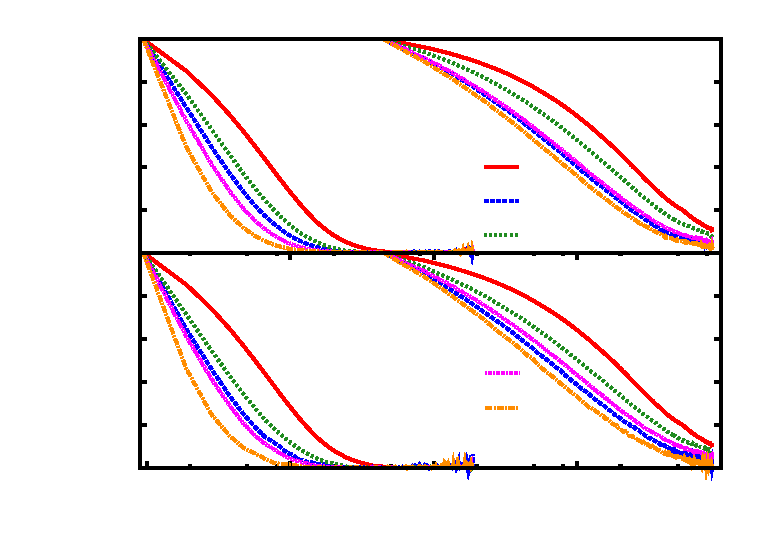
\includegraphics{./isf_qlm_normed}}%
    \gplfronttext
  \end{picture}%
\endgroup
}
	\caption{Comparison of the particle-wise time autocorrelation function of $g_\ell$ (top) and $G_\ell$ (bottom) for normal liquid (left) and deeply supercooled liquid (right). All functions are normalized by their value at $\delta t$, which is an approximation of their respective Debye-Waller factor. The self \acs{ISF} (continuous lines) is normalized in the same way and plotted each time as a reference.}
	\label{fig:Qlm_corr}
\end{figure}

With this representation, the relaxation time can be directly approximated by the time $\tau$ so that $g_\ell(\tau)=e^{-1}$. For all $\ell$, the bond order relaxation time is smaller than the usual structural relaxation time $\tau_\alpha$. Among the bond orders, the 6-fold symmetry always has the largest relaxation time. This justifies our focus on the 6-fold invariants that catches the long-lived structures.

\begin{figure}
	\centering
	\resizebox{0.8\textwidth}{!}{% GNUPLOT: LaTeX picture with Postscript
\begingroup
  \makeatletter
  \providecommand\color[2][]{%
    \GenericError{(gnuplot) \space\space\space\@spaces}{%
      Package color not loaded in conjunction with
      terminal option `colourtext'%
    }{See the gnuplot documentation for explanation.%
    }{Either use 'blacktext' in gnuplot or load the package
      color.sty in LaTeX.}%
    \renewcommand\color[2][]{}%
  }%
  \providecommand\includegraphics[2][]{%
    \GenericError{(gnuplot) \space\space\space\@spaces}{%
      Package graphicx or graphics not loaded%
    }{See the gnuplot documentation for explanation.%
    }{The gnuplot epslatex terminal needs graphicx.sty or graphics.sty.}%
    \renewcommand\includegraphics[2][]{}%
  }%
  \providecommand\rotatebox[2]{#2}%
  \@ifundefined{ifGPcolor}{%
    \newif\ifGPcolor
    \GPcolortrue
  }{}%
  \@ifundefined{ifGPblacktext}{%
    \newif\ifGPblacktext
    \GPblacktexttrue
  }{}%
  % define a \g@addto@macro without @ in the name:
  \let\gplgaddtomacro\g@addto@macro
  % define empty templates for all commands taking text:
  \gdef\gplbacktext{}%
  \gdef\gplfronttext{}%
  \makeatother
  \ifGPblacktext
    % no textcolor at all
    \def\colorrgb#1{}%
    \def\colorgray#1{}%
  \else
    % gray or color?
    \ifGPcolor
      \def\colorrgb#1{\color[rgb]{#1}}%
      \def\colorgray#1{\color[gray]{#1}}%
      \expandafter\def\csname LTw\endcsname{\color{white}}%
      \expandafter\def\csname LTb\endcsname{\color{black}}%
      \expandafter\def\csname LTa\endcsname{\color{black}}%
      \expandafter\def\csname LT0\endcsname{\color[rgb]{1,0,0}}%
      \expandafter\def\csname LT1\endcsname{\color[rgb]{0,1,0}}%
      \expandafter\def\csname LT2\endcsname{\color[rgb]{0,0,1}}%
      \expandafter\def\csname LT3\endcsname{\color[rgb]{1,0,1}}%
      \expandafter\def\csname LT4\endcsname{\color[rgb]{0,1,1}}%
      \expandafter\def\csname LT5\endcsname{\color[rgb]{1,1,0}}%
      \expandafter\def\csname LT6\endcsname{\color[rgb]{0,0,0}}%
      \expandafter\def\csname LT7\endcsname{\color[rgb]{1,0.3,0}}%
      \expandafter\def\csname LT8\endcsname{\color[rgb]{0.5,0.5,0.5}}%
    \else
      % gray
      \def\colorrgb#1{\color{black}}%
      \def\colorgray#1{\color[gray]{#1}}%
      \expandafter\def\csname LTw\endcsname{\color{white}}%
      \expandafter\def\csname LTb\endcsname{\color{black}}%
      \expandafter\def\csname LTa\endcsname{\color{black}}%
      \expandafter\def\csname LT0\endcsname{\color{black}}%
      \expandafter\def\csname LT1\endcsname{\color{black}}%
      \expandafter\def\csname LT2\endcsname{\color{black}}%
      \expandafter\def\csname LT3\endcsname{\color{black}}%
      \expandafter\def\csname LT4\endcsname{\color{black}}%
      \expandafter\def\csname LT5\endcsname{\color{black}}%
      \expandafter\def\csname LT6\endcsname{\color{black}}%
      \expandafter\def\csname LT7\endcsname{\color{black}}%
      \expandafter\def\csname LT8\endcsname{\color{black}}%
    \fi
  \fi
  \setlength{\unitlength}{0.0500bp}%
  \begin{picture}(7200.00,5040.00)%
    \gplgaddtomacro\gplbacktext{%
      \csname LTb\endcsname%
      \put(264,2842){\makebox(0,0)[r]{\strut{}$0.3$}}%
      \put(264,3165){\makebox(0,0)[r]{\strut{}$0.4$}}%
      \put(264,3487){\makebox(0,0)[r]{\strut{}$0.5$}}%
      \put(264,3809){\makebox(0,0)[r]{\strut{}$0.6$}}%
      \put(264,4131){\makebox(0,0)[r]{\strut{}$0.7$}}%
      \put(264,4454){\makebox(0,0)[r]{\strut{}$0.8$}}%
      \put(264,4776){\makebox(0,0)[r]{\strut{}$0.9$}}%
      \put(396,2300){\makebox(0,0){\strut{}}}%
      \put(1689,2300){\makebox(0,0){\strut{}}}%
      \put(2983,2300){\makebox(0,0){\strut{}}}%
      \put(-374,2548){\makebox(0,0){\strut{}$\frac{G_\ell(t)}{g_\ell(t)}$}}%
      \put(3819,3648){\rotatebox{-270}{\makebox(0,0){\strut{}}}}%
      \put(1998,2234){\makebox(0,0){\strut{}}}%
      \put(1998,4666){\makebox(0,0){\strut{}}}%
      \put(1998,4665){\makebox(0,0){\strut{}}}%
      \put(-528,2410){\makebox(0,0)[l]{\strut{}}}%
      \put(1013,4212){\makebox(0,0){\strut{}$\ell=4$}}%
    }%
    \gplgaddtomacro\gplfronttext{%
    }%
    \gplgaddtomacro\gplbacktext{%
      \csname LTb\endcsname%
      \put(3468,2842){\makebox(0,0)[r]{\strut{}}}%
      \put(3468,3165){\makebox(0,0)[r]{\strut{}}}%
      \put(3468,3487){\makebox(0,0)[r]{\strut{}}}%
      \put(3468,3809){\makebox(0,0)[r]{\strut{}}}%
      \put(3468,4131){\makebox(0,0)[r]{\strut{}}}%
      \put(3468,4454){\makebox(0,0)[r]{\strut{}}}%
      \put(3468,4776){\makebox(0,0)[r]{\strut{}}}%
      \put(3600,2300){\makebox(0,0){\strut{}}}%
      \put(4893,2300){\makebox(0,0){\strut{}}}%
      \put(6187,2300){\makebox(0,0){\strut{}}}%
      \put(7023,3648){\rotatebox{-270}{\makebox(0,0){\strut{}}}}%
      \put(5202,2234){\makebox(0,0){\strut{}}}%
      \put(5202,4666){\makebox(0,0){\strut{}}}%
      \put(5202,4665){\makebox(0,0){\strut{}}}%
      \put(3336,2410){\makebox(0,0)[l]{\strut{}}}%
      \put(4217,4212){\makebox(0,0){\strut{}$\ell=6$}}%
    }%
    \gplgaddtomacro\gplfronttext{%
    }%
    \gplgaddtomacro\gplbacktext{%
      \csname LTb\endcsname%
      \put(264,963){\makebox(0,0)[r]{\strut{}$0.3$}}%
      \put(264,1223){\makebox(0,0)[r]{\strut{}$0.4$}}%
      \put(264,1482){\makebox(0,0)[r]{\strut{}$0.5$}}%
      \put(264,1741){\makebox(0,0)[r]{\strut{}$0.6$}}%
      \put(264,2000){\makebox(0,0)[r]{\strut{}$0.7$}}%
      \put(264,2260){\makebox(0,0)[r]{\strut{}$0.8$}}%
      \put(264,2519){\makebox(0,0)[r]{\strut{}$0.9$}}%
      \put(396,484){\makebox(0,0){\strut{}$0.01$}}%
      \put(1689,484){\makebox(0,0){\strut{}$0.1$}}%
      \put(2983,484){\makebox(0,0){\strut{}$1$}}%
      \put(3819,1611){\rotatebox{-270}{\makebox(0,0){\strut{}}}}%
      \put(1998,154){\makebox(0,0){\strut{}$t/\tau_\alpha$}}%
      \put(1998,2409){\makebox(0,0){\strut{}}}%
      \put(1998,2408){\makebox(0,0){\strut{}}}%
      \put(-528,110){\makebox(0,0)[l]{\strut{}}}%
      \put(1013,2065){\makebox(0,0){\strut{}$\ell=8$}}%
    }%
    \gplgaddtomacro\gplfronttext{%
      \csname LTb\endcsname%
      \put(1488,842){\makebox(0,0)[r]{\strut{}$\phi=0.497$}}%
      \csname LTb\endcsname%
      \put(1488,1062){\makebox(0,0)[r]{\strut{}$\phi=0.535$}}%
      \csname LTb\endcsname%
      \put(1488,1282){\makebox(0,0)[r]{\strut{}$\phi=0.555$}}%
      \csname LTb\endcsname%
      \put(1488,1502){\makebox(0,0)[r]{\strut{}$\phi=0.576$}}%
    }%
    \gplgaddtomacro\gplbacktext{%
      \csname LTb\endcsname%
      \put(3468,963){\makebox(0,0)[r]{\strut{}}}%
      \put(3468,1223){\makebox(0,0)[r]{\strut{}}}%
      \put(3468,1482){\makebox(0,0)[r]{\strut{}}}%
      \put(3468,1741){\makebox(0,0)[r]{\strut{}}}%
      \put(3468,2000){\makebox(0,0)[r]{\strut{}}}%
      \put(3468,2260){\makebox(0,0)[r]{\strut{}}}%
      \put(3468,2519){\makebox(0,0)[r]{\strut{}}}%
      \put(3600,484){\makebox(0,0){\strut{}$0.01$}}%
      \put(4893,484){\makebox(0,0){\strut{}$0.1$}}%
      \put(6187,484){\makebox(0,0){\strut{}$1$}}%
      \put(7023,1611){\rotatebox{-270}{\makebox(0,0){\strut{}}}}%
      \put(5202,154){\makebox(0,0){\strut{}$t/\tau_\alpha$}}%
      \put(5202,2409){\makebox(0,0){\strut{}}}%
      \put(5202,2408){\makebox(0,0){\strut{}}}%
      \put(3336,110){\makebox(0,0)[l]{\strut{}}}%
      \put(4217,2065){\makebox(0,0){\strut{}$\ell=10$}}%
    }%
    \gplgaddtomacro\gplfronttext{%
    }%
    \gplbacktext
    \put(0,0){\includegraphics{./Qlm_qlm_correl_ratio_bis}}%
    \gplfronttext
  \end{picture}%
\endgroup
}
	\caption{The ratio $G_\ell(t)/g_\ell(t)$ for $\ell=4,6,8,10$ at different supercooling. A constant ratio would indicate that among the structures of $\ell$-fold symmetry, the periodic and aperiodic structures are playing the same role in the relaxation. A decreasing ratio indicates that the periodic structures decay more rapidly than the aperiodic ones. Note that the time scale is normalised by $\tau_\alpha$ to show when each decay appends during the relaxation of the system.}
	\label{fig:Qlm_qlm_correl_ratio}
\end{figure}

To distinguish between the decay of the periodic and aperiodic structures, we investigate the ratio $G_\ell(t)/g_\ell(t)$ (see \FigureRef{fig:Qlm_qlm_correl_ratio}). $g_\ell(t)$ catches the lifetime of all structures with strong $\ell$-fold symmetry; $G_\ell(t)$ catches only the lifetime of the (locally) periodic structures. Intuitively their ratio is smaller than one and should increase with time if the crystal-like structures live longer than the aperiodic ones.

At low supercooling, the $G_6(t)/g_6(t)$ ratio decreases with time. This means that the icosahedral order is more stable than the crystal-like order for these densities. However for $\ell=8$, the ratio increases, showing that periodic structures (our crystal-like bond ordered clusters) are longer-lived than aperiodic $8$-fold symmetric structures. The decrease of the ratio for $\ell=4$ and $\ell=10$ merely indicates that in these symmetries structures larger than the first shell are not stable.

Approaching the glass transition, the ratio $G_\ell(t)/g_\ell(t)$ has much higher values than at low supercooling: most of the long lived structures are periodic. However, this predominance gets eroded at medium time scales ($\sim\tau_\alpha/10$) for $\ell=6,10$, indicating that icosahedral order still plays an important role. Nevertheless, at times longer than $\tau_\alpha$ the ratio increases for all $\ell$ except $\ell=10$ where it stops decreasing to stay constant. This means that really long-lived structures, lasting more than the relaxation time of the system, are the crystal-like bond order we discussed in \SectionRef{sec:X_order}. 

\section{Summary and Discussion}

From our observations a unified picture emerges for the structure of a hard sphere supercooled liquid. From the great variety of possible local structures we showed that only two types of mutually exclusive order predominate and thus both in number and in lifetime: 
\begin{itemize}
	\item The icosahedral order is the most important at moderate densities (even for $\phi<\phi_X$) and at times shorter or comparable to the relaxation time of the system. Icosahedra form a network that finally percolates through the system but cannot cover space.
	\item The crystal-like order appears faintly when crossing $\phi_X$ and becomes important at high density. It forms compact clusters closely related to \ac{FCC} ordering but without the density gain characteristic of crystal nucleus. It's correlation length $\xi_6$ diverges when approaching ideal glass transition $\phi_0$. At high density, the crystal-like bond ordered clusters are the longest-lived structures of the system with a characteristic lifetime of a few $\tau_\alpha$.
\end{itemize}

Because we deal with hard spheres, we are sure that the driving force of ordering is the gain in vibrational entropy. More precisely, we showed that crystal-like bond ordering gives more free volume for each ordered particle, whereas icosahedral ordering compresses the central particle of the icosahedron to leave more free volume to its neighbours. This last effect favours the interlocking and aggregation of icosahedra.

This rather simple picture may be generalised to systems with a potential energy if we understand how the potential effects the entropic balance between crystal-like and icosahedral ordering.